% AgriOcc v2: Elsevier CAS single-column, compile with XeLaTeX.
% Let the CAS/STIX math fonts handle symbols when ctex loads fontspec.
\PassOptionsToPackage{no-math}{fontspec}
\documentclass[a4paper,fleqn]{cas-sc}
\usepackage[UTF8]{ctex}
\usepackage[authoryear]{natbib}
% CAS/STIX fills most XeTeX math families; avoid bm's extra preallocation.
\chardef\bmmax=0
\chardef\hmmax=0
\usepackage{bm,tikz,enumitem,threeparttable,xcolor}
\usetikzlibrary{arrows.meta,positioning,fit}
\hypersetup{colorlinks=true,linkcolor=black,citecolor=black,urlcolor=blue}
\ExplSyntaxOn
\bool_gset_true:N \g_stm_nologo_bool
\ExplSyntaxOff
\newcommand{\R}{\mathbb{R}}
\newcommand{\B}{\mathcal{B}}
\newcommand{\V}{\mathcal{V}}
\newcommand{\I}{\mathcal{I}}
\newcommand{\softmax}{\operatorname{softmax}}
\newcommand{\IoU}{\operatorname{IoU}}
\newcommand{\mIoU}{\operatorname{mIoU}}
\newcommand{\temp}[1]{\textcolor{blue!65!black}{#1\textsuperscript{\ensuremath{\dagger}}}}
\begin{document}
\let\WriteBookmarks\relax
\def\floatpagepagefraction{1}
\def\textpagefraction{.001}
\shorttitle{AgriOcc}
\shortauthors{He, Jin and Liu}
\title[mode=title]{AgriOcc：面向农业机器人的作物感知三维语义占用预测}
\author[1]{Lei He}
\author[1]{Jing Jin}[orcid=0000-0001-7753-7656]
\cormark[1]
\ead{jinjinghit@hit.edu.cn}
\author[2]{Yi Liu}
\affiliation[1]{organization={School of Astronautics, Harbin Institute of Technology},
 city={Harbin},postcode={150001},country={China}}
\affiliation[2]{organization={Zhengzhou Advanced Research Institute of Harbin Institute of Technology},
 city={Zhengzhou},postcode={450000},country={China}}
\begin{abstract}
农业机器人需要同时理解作物、土壤、可通行区域与障碍物的三维空间关系，而二维作物行检测和图像分割难以直接提供统一的空间表示。
本文提出 AgriOcc，从正前、左前与右前三路 RGB 图像预测机器人前方 $15\times15\times5\,\mathrm{m}$ 范围的六类语义占用。
针对农业场景中植株与地面结构各向异性、作物监督在场景和样本间分布不均的问题，
AgriOcc 在保留 BEVFormer 可变形自注意力骨架的基础上，设计农业结构自适应混合专家解码器 Agri-AMoE，并提出作物感知采样策略 CropSample。
Agri-AMoE 将 BEV 表征提升为三维特征体，先以通道注意力增强特征，再利用空间显著性和梯度能量在局部平面、垂直结构和大范围上下文专家之间自适应路由。
CropSample 以少量配额替换增加含作物样本的训练曝光，在不增多训练数据的前提下可有效提高模型对作物的感知能力。
针对农业语义占用数据稀缺且采集成本高的问题，本文构建了农业多视角仿真数据集 AgriOcc-Dataset。
它包含 298 个序列、38,862 帧样本，覆盖十种作物、三个生长阶段、五个时段和两类天气。
在该数据集上，AgriOcc 取得 64.08\% mIoU 和 39.38\% 作物 IoU，显著优于其他先进的三维语义占用方法。
在真实越野数据集 ORAD-3D 上以AgriOcc进行目标域适配也表现出显著的效率和性能提升。另外在体素分辨率迁移实验和真实农田的零样本预测中，AgriOcc也展现出良好的泛化能力。
大量实验表明，AgriOcc 具备良好的农业场景理解与真实环境迁移能力，为农业移动机器人的三维视觉导航提供了兼顾精度与训练开销的新路径。
\end{abstract}
\begin{keywords}
农业机器人 \sep 三维语义占用 \sep 混合专家 \sep 作物感知采样 \sep 分辨率迁移
\end{keywords}
\maketitle
\section{引言}\label{sec:intro}
农业机器人在田间执行巡检、植保、收获运输和自主导航时，需要同时理解作物、垄沟、土壤、
可通行区域与突发障碍物的空间关系。现有视觉导航系统通常采用模块化流程：
先通过作物行识别、道路或可通行区域分割得到二维结果，再经几何拟合、
坐标变换和规则后处理生成导航约束\citep{nkwochaComprehensiveReviewSensing2025,baiVisionbasedNavigationGuidance2023}。
该流程存在两个限制：
其一，二维感知、几何恢复和控制坐标变换彼此分离，不同阶段的误差容易累积；
其二，基于二维感知的范式往往需要额外依赖激光雷达或深度相机来测距和判断物体的位姿。
对于农场中大小不一的障碍物、行人，二维像素级结果也难以表达高度、遮挡后空间。
其三，基于的二维感知技术的系统往往需要多种感知模型配合使用，带来额外的训练与调试成本。

三维语义占用预测以机器人自身坐标系中的规则体素网格统一表示环境，每个体素给出语义类别。
首先，它能够将自由空间、地面、作物和障碍物以统一接口提供给后续通行性分析、碰撞检查和视觉导航。
其次，它无需投影、滤波、栅格化等后处理，直接输出结构化空间表示，多相机空间一致性更好。
此外，可根据周围的语义信息预测被遮挡区域，而深度图则仅能预测每条光线上最近的被占用点，无法恢复三维场景中被遮挡的部分。
与二维语义图相比，占用表示显式保留物体高度及空间邻接关系，能够为后续通行性评估、碰撞检查和路径规划提供同一份环境描述。
自动驾驶研究已证明，Lift--Splat--Shoot 等显式提升方法\citep{philion2020lift,huang2021bevdet,li2022bevdepth}，
以及 DETR3D、PETR 和 BEVFormer 等查询式方法\citep{wang2022detr3d,li2022petr,li2022bevformer}，
都可从多相机图像学习几何一致的鸟瞰表征；该表征还能扩展至稠密占用\citep{wei2023surroundocc,wang2023openoccupancy}、
时序场景预测和规划\citep{zheng2024occworld,mei2025irwm}。
这些方法常设定六路环视相机、面向全向道路交通场景，并使用较大时空范围与模型规模。
而农业机器人则通常配备低算力平台，多在相对静态、前向作业的田间环境中运行。
因此本文聚焦农业机器人最常见的前向作业视野：输入正前、左前和右前三路相机，
预测前方 $20\,$m 的三维语义占用。

然而，将三维语义占用方法直接迁移到农业任务中仍面临三项关键挑战。
首先，农田的空间结构具有明显方向性：地面和作物行沿水平面延伸，冠层、茎秆和障碍物又具有不同的垂直形态。
若每个 BEV 单元仅通过独立 MLP 输出所有高度的类别，相邻植株与地面边界容易被平滑。
其次，场景中的大量自由空间和背景地面，使不同样本提供的作物监督量差异显著。
单纯提高作物损失权重并不等价于增加有效作物观测，过强的重加权还可能扩大作物假阳性。
最后，真实农业数据受到季节、作物生长期、地块变化、传感器配置和标注成本等限制，难以支持覆盖多种田间条件的系统研究。
现有研究往往也只针对一种作物，难以进行跨地域、跨作物种类的泛化性研究。

为建立全面、多样、可控的训练与评测环境，本文首先基于 Unreal Engine 5 构建了 AgriOcc-Dataset：包含 298 个完整序列、38,862 帧多视角样本，
涵盖 10 种作物、3 个生长阶段、5 个时段及两类天气条件的农业语义占用数据。
之后，本文提出了面向农业移动机器人的三维语义占用网络 AgriOcc。如图\ref{fig:overview}所示，ResNet--FPN 首先提取多尺度图像特征，
BEVFormer  式编码器再通过可变形自注意力与图像空间交叉注意力建立统一 BEV 表征。
我们保留原 Temporal Self-Attention（TSA）的当前帧可变形空间聚合能力。
随后，Agri-AMoE 将 BEV 提升为三维特征体，根据局部梯度能量和空间显著性融合三个各向异性专家，输出六类占用。
训练阶段的 CropSample 从当前预测范围内统计作物体素，以小比例配额替换增强含作物样本的曝光；它在不增加每轮样本数，也不改变推理网络的前提下显著增强了模型对作物的感知能力。

\begin{figure}[pos=htbp]
\centering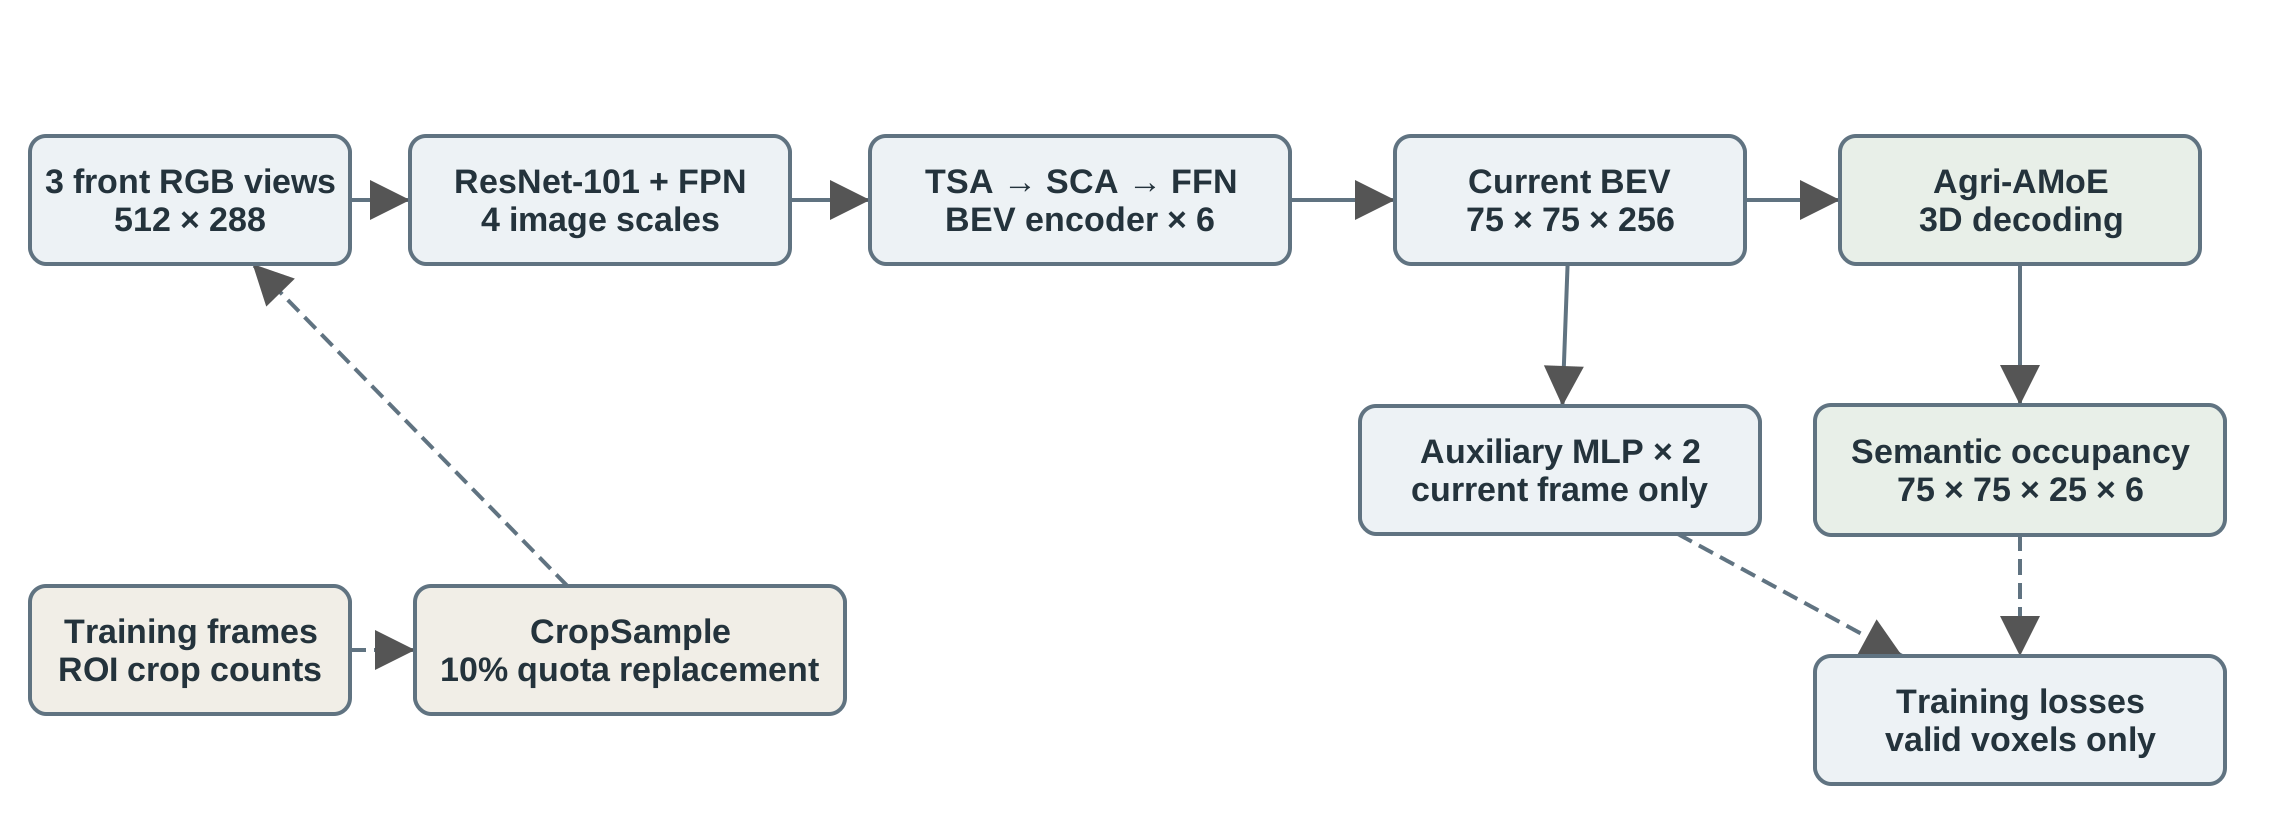
\includegraphics[width=\linewidth]{overview.png}
\caption{AgriOcc 总体架构。实线表示当前帧推理路径，虚线表示训练监督与 CropSample 数据组织。六层 BEV 编码器由 TSA、图像空间交叉注意力和前馈更新组成；最终 Agri-AMoE 分支输出占用，两路辅助分支提供训练监督。}
\label{fig:overview}
\end{figure}

本文的主要贡献如下：
\begin{enumerate}[leftmargin=1.8em]
\item 构建面向农业机器人三维语义占用的仿真数据集 AgriOcc-Dataset：包含 298 个序列、38.8k 个样本，
在机器人自身坐标系下提供六类前方环境体素标注，并给出可参数化的数据采集与自动标注流程；
\item  提出 AgriOcc，据我们所知首个面向农业移动机器人前向作业视野的三维语义占用预测模型。
它通过端到端学习将三路前视 RGB 图像映射为前方空间的稠密语义体素，提供统一的农业环境三维表征；
\item 提出面向农业结构的 Agri-AMoE 解码器，以三维梯度能量和空间显著性驱动各向异性专家融合，增强统一 BEV 到语义占用的结构化解码。
\item 提出 CropSample 训练策略，在固定训练长度下提高模型对作物的感知能力，显著提高作物IoU。
\end{enumerate}
\section{相关工作}\label{sec:related}
\paragraph{多相机 BEV 感知}
鸟瞰（bird's-eye-view, BEV）表征将多相机图像中的视觉证据映射到机器人或车辆坐标系的俯视平面，使不同视角的观测能够在统一空间网格中进行融合、推理和规划。
以 BEV 为中间表征的视觉感知方法通过预定义空间查询把多相机图像特征对齐到该统一坐标系。
显式提升范式将图像特征沿深度分布投影至 BEV，代表性工作包括 Lift--Splat--Shoot、BEVDet、
BEVDepth 和 BEVStereo\citep{philion2020lift,huang2021bevdet,li2022bevdepth,li2022bevstereo}；
MatrixVT 则进一步讨论了高效的多相机到 BEV 变换\citep{zhou2022matrixvt}。
查询式方法则利用三维参考点、位置嵌入或跨视图变换直接读取相机特征\citep{wang2022detr3d,li2022petr,liu2023petrv2,li2023fbbev}，
并可在共享 BEV 中融合多模态信息\citep{liu2023bevfusion}。
BEVFormer 进一步以空间交叉注意力和时序自注意力建立 BEV 查询之间的几何关联\citep{li2022bevformer}。
这些方法为统一坐标系下的视觉感知奠定基础。

\paragraph{三维占用预测与高效表征}
视觉三维占用将自由空间和语义实体编码为稠密或压缩的体素场。MonoScene、TPVFormer 和 VoxFormer 分别从单目特征提升、
三平面表征和可见稀疏体素出发完成场景补全\citep{cao2022monoscene,huang2023tpvformer,li2023voxformer}；
SurroundOcc 与 OpenOccupancy 推动了多相机稠密占用预测和环视基准的发展\citep{wei2023surroundocc,wang2023openoccupancy}。
由于三维体素的计算代价随空间分辨率快速增长，后续工作从局部--全局结构、
紧凑或由粗到细的查询、稀疏交互，以及高效解码和渲染监督等方向降低开销\citep{zhang2023occformer,ma2024cotr,wang2024panoocc,liu2024sparseocc,tang2024sparseocc,yu2023flashocc,pan2024renderocc}。
占用表征也进一步扩展为时序世界模型：BEVDet4D、OccWorld、IR-WM 与 ForecastOcc 分别
利用跨帧 BEV、离散场景 token 或历史图像观测预测动态环境和未来状态\citep{huang2022bevdet4d,zheng2024occworld,mei2025irwm,mohan2026forecastocc}。
这些研究验证了占用作为统一空间接口的价值，但其普遍面向全向交通环境，
依赖更广的相机覆盖或历史运动信息。

\paragraph{农业与越野三维感知数据}
城市三维感知的常用数据集包括 KITTI\citep{geiger2012kitti}、SemanticKITTI\citep{behley2019semantickitti} 和 nuScenes\citep{caesar2020nuscenes}，
但它们的传感器布置、类别构成和道路结构与农田不同。
农业场景中的公开数据多面向作物行检测、二维语义分割、实例分割或特定作业目标，难以同时提供多相机标定和稠密三维语义体素；
越野方向的 RELLIS-3D\citep{jiang2020rellis} 也主要服务于多模态分割与建图。
虚拟驾驶平台 CARLA\citep{dosovitskiy2017carla} 及领域随机化\citep{tobin2017domainrandomization,peng2018sim2real}、
语义一致域适应\citep{hoffman2018cycada} 说明仿真环境可以极大地缓解真实世界数据采集成本高、周期长的难题，
这一点在农业场景中尤为突出。
在真实越野方向，ORAD-3D 提供涵盖农田、林地、草地和道路等场景的三维占用
基准\citep{chen2025orad3d}，为本文提供了真实场景下的验证途径。
需要说明的是，现有农业与越野三维感知工作多基于激光雷达或单目相机，
其传感器配置与任务定义均不同于本文的多路前视相机稠密语义占用预测，
因此未纳入本文的实验对比协议。据我们所知，目前面向农业机器人前向作业视野、
以多路前视相机直接输出机器人坐标系稠密三维语义占用的方法仍属空白。
\section{方法}\label{sec:method}

\subsection{任务定义}\label{sec:task}
本文聚焦农业机器人最常见的前向作业视野：输入正前、左前和右前三路相机，预测前方 $20\,$m 的三维语义占用。
给定时刻 $t$ 的三路同步图像 $\I_t=\{I_t^{\mathrm{FL}},I_t^{\mathrm{F}},I_t^{\mathrm{FR}}\}$、
相机内外参和机器人坐标系，目标是在前向空间
\begin{equation}
\B=[0,20]\times[-10,10]\times[-2,3]~\mathrm{m}
\end{equation} 
中预测语义占用。体素分辨率为 $0.2~\mathrm{m}$，因此输出网格为 $100\times100\times25$。
每个有效体素 $v\in\V$ 的标签 $y_v\in\{0,\ldots,5\}$ 分别表示自由空间、
作物、土壤地面、可通行区域（drivable）、其他植被与其他障碍物六类。

\subsection{仿真数据采集系统与AgriOcc-Dataset}\label{sec:dataset_construction}
\subsubsection{农田仿真数据采集系统}\label{sec:synthetic}
为缓和农业场景作物种类繁多、数据采集时间跨度大等问题带来的农机数据采集困难，
本文首先基于 Unreal Engine 5 构建可参数化农场仿真环境，其流程如图\ref{fig:synthetic}所示。
场景包含农田、道路、地表、作物、房屋、围栏等常见元素，并依据作物种植边界和行株距对作物实例进行网格化布设。
针对每个场景，系统先从作物类别与生长阶段中选择对应资产。然后在保持田间结构合理和满足农艺先验约束的前提下，
对植株尺度、朝向、行株距、位置扰动及缺株比例进行随机化，从而模拟不同长势、密度与田间分布形态。

之后在无人拖拉机车体上配置左前、正前和右前三个同步 RGB 传感器，形成面向行进方向的多视角观测。
传感器的安装高度、视场角、分辨率及采样频率可统一配置；采集过程中同步记录相机内外参数、车辆位姿、
速度及当前场景配置，保证图像、车辆状态与占用真值在时间和空间上的一致性。
\begin{figure}[pos=htbp]
\centering
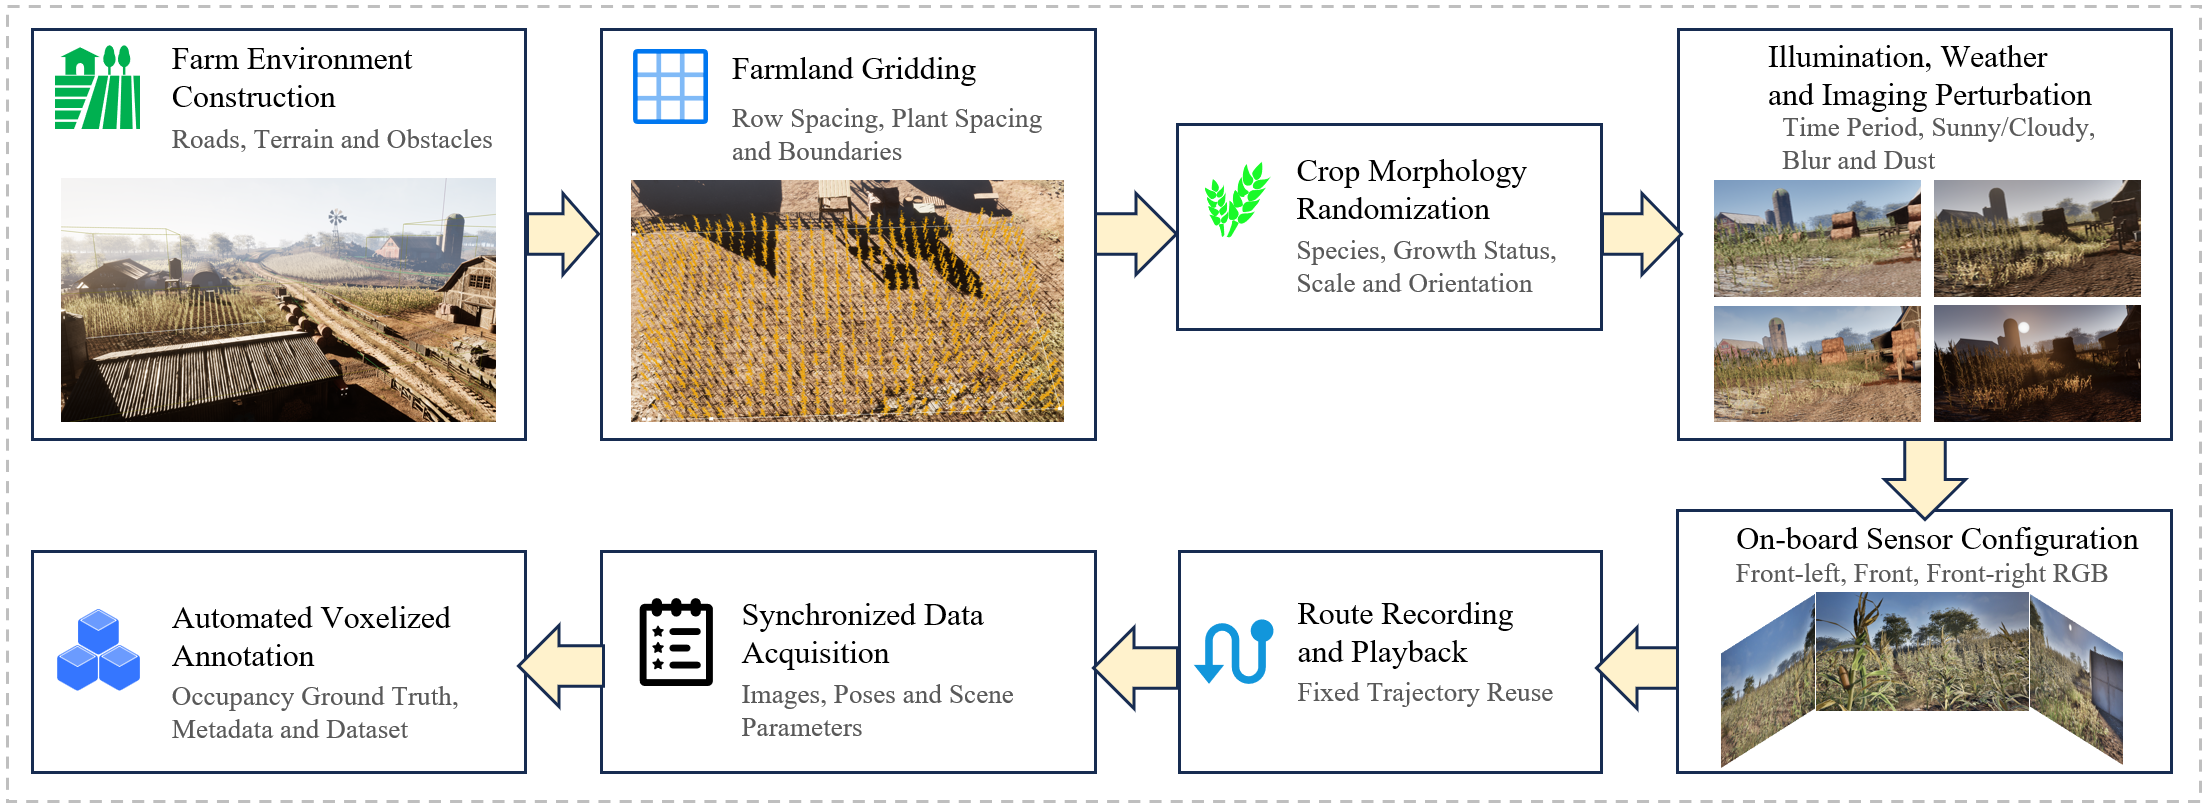
\includegraphics[width=1\linewidth]{synthetic.png}
\caption{农田仿真数据采集系统的构建流程。}
\label{fig:synthetic}
\end{figure}

采集数据时首先录制拖拉机在农田中的若干行驶轨迹，再针对不同的作物种类、生长阶段、光照时段和天气组合重放路线，
实现多样的农田场景与运动轨迹的组合。为缩小仿真与真实采集之间的外观差异，
系统进一步以设定概率在 RGB 图像上施加运动模糊、镜头污渍和扬尘颗粒等成像扰动。
数据标注方面，与 nuScenes 等真实采集数据集不同，仿真引擎可直接导出相机位姿、场景语义和体素占用状态，
无需进行人工逐帧点云语义标注、多帧点云时空配准及体素标签生成等复杂流程。
对每一帧数据，系统将车辆局部坐标系下的前方空间划分为规则三维体素网格，并基于场景几何与语义标签自动生成稠密占用真值。
原始环境语义根据任务需求归并为自由空间、作物、土壤地面、可通行区域、其他植被和其他障碍物六类，
最终，每个样本由三视角 RGB 图像、对应的三维语义占用标签以及位姿和场景参数元数据组成，从而形成可用于视觉占用预测训练与评估的农田多模态数据集。
\subsubsection{AgriOcc-Dataset}\label{sec:agriocc_dataset}
基于上述流程，我们构建了面向田间农业机器人的多视角三维语义占用数据集 AgriOcc-Dataset。
每个序列包含正前、左前和右前三视角的同步 RGB 图像、相机内外参、机器人位姿、语义占用标签及有效体素掩码。
标签在加载阶段统一映射为 free、crop、soil\_ground、drivable、other\_vegetation 和 other\_obstacle 六类，并在机器人自身坐标系中生成前方体素监督。

数据集包含 298 个仿真行驶序列，原始记录频率为 10 Hz，共约 194k 帧。
为避免相似场景大量重复，我们下采样至 2 Hz，得到 38.8k 个样本。
其中 248 个序列（32,385 帧）用于训练，50 个序列（6,477 帧）用于验证。
数据覆盖 cabbage、carrot、corn、cucumber、potato、radish、redbeet、sunflower、tomato 和 wheat 十种作物；
每种作物进一步包含 early、mid 和 mature 三个生长阶段，并覆盖 dawn、morning、noon、evening 和 night 五个时段，
以及 cloudy 与 sunny 两类天气。图\ref{fig:crop_distribution}给出了总体数据集的作物组成。

\begin{figure}[pos=htbp]
\centering
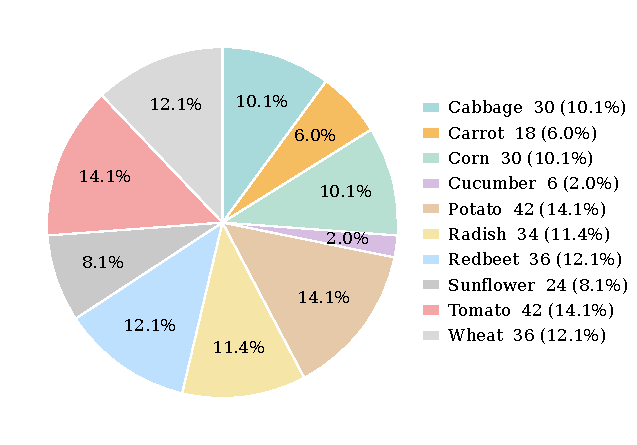
\includegraphics[width=0.5\linewidth]{crop_distribution.pdf}
\caption{AgriOcc-Dataset 的作物组成。扇区面积表示各作物的占比。}
\label{fig:crop_distribution}
\end{figure}

\begin{figure}[pos=htbp]
\centering
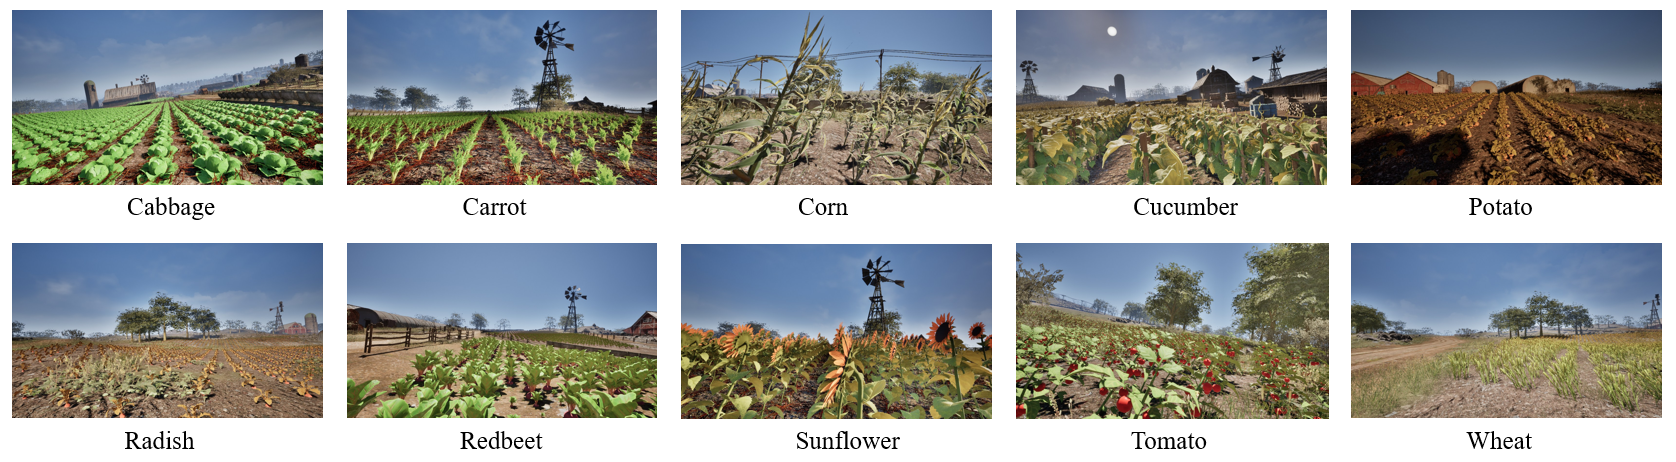
\includegraphics[width=\linewidth]{dataset.png}
\caption{AgriOcc-Dataset 中十种作物的场景示例。}
\label{fig:dataset}
\end{figure} 

\subsection{AgriOcc 总体架构}\label{sec:architecture}
图\ref{fig:overview}展示整体流程。
输入张量为 $B\times3\times3\times288\times512$，其中 $B$ 为 batch size，一个样本包含前视、左前、右前3个相机、3个颜色通道，图像分辨率为512*288.
图像编码时合并 batch 与相机维，ResNet-101--FPN 输出四级、每级 256 通道的特征。
之后，六层 BEV 编码器以 $75\times75$ 个查询聚合这些图像特征，经逐层自注意力与空间交叉注意力更新后，
输出 $75\times75$、通道数为 256 的 BEV token；
由 Agri-AMoE 将 BEV token 提升为三维特征体并预测 25 个高度位置上的六类 logits。
最终输出为 $B\times75\times75\times25\times6$ logits，按类别取最大值得到语义网格。
CropSample 用于在训练期间增加作物体素的曝光率。

\subsection{当前帧 BEV 编码}\label{sec:bev}
农业三视角投影存在遮挡、视野边界与局部观测缺失，直接把各位置独立投影到占用头容易破坏空间一致性。
本文借鉴 BEVFormer 的基本架构\citep{li2022bevformer}，以 BEV 自适应采样和跨视角投影交替更新查询。
每层执行
\begin{equation}
\begin{aligned}
\widetilde{\bm Q}^{l}&=\operatorname{LN}\!\left(\operatorname{TSA}(\bm Q^{l-1})\right),\\
\widehat{\bm Q}^{l}&=\operatorname{LN}\!\left(\operatorname{SCA}(\widetilde{\bm Q}^{l},\{\bm F_s\},\Pi)\right),\\
\bm Q^l&=\operatorname{LN}\!\left(\widehat{\bm Q}^{l}+\operatorname{FFN}(\widehat{\bm Q}^{l})\right),
\end{aligned}
\end{equation}
其中 $l=1,\ldots,6$，$\bm F_s$ 为第 $s$ 级图像特征，$\Pi$ 为各相机投影关系，LN 为层归一化；TSA 与空间交叉注意力 SCA 均包含其内部残差。

原 TSA 在没有历史 BEV 时将当前查询复制到两个内部 value 槽，并依据查询预测少量二维采样偏移与注意力权重。
因此，它承担当前 BEV 上的可变形空间交互。我们留该模块来复用其成熟的自适应空间聚合机制。
SCA 则把柱状参考点投影至三幅图像，在有效视角和多个特征尺度上采样并汇聚视觉证据。

\subsection{农业结构自适应混合专家解码}\label{sec:amoe}
农田占用空间具有显著的各向异性：作物行与垄沟在地平面上呈现长程连续和周期性交替，
作物冠层、土壤和障碍物又在高度方向具有不同的边界形态。
特别是株间空隙和作物与自由空间的边界往往只占少量体素，
若将二维 BEV token 独立地直接映射为各高度类别，
解码器难以协调相邻位置的平面细节与垂直结构，预测容易在细粒度区域发生过度平滑。
因而，最终占用头不仅需要恢复高度维度，还应按局部三维结构的复杂度自适应地选择合适的感受野与方向建模方式。

受文献\citep{shi2026oneocc}将混合专家引入占用解码的启发，本文设计农业结构自适应混合专家三维占用解码器（Agri-AMoE）。
与在通用城市场景下定义专家不同，本文依据农田空间在平面、垂直与上下文三个方向上的
各向异性结构来定义专家形态，并以可解释的梯度能量作为路由信号，
使专家分工与作物行、垄沟和冠层等农业结构直接对应。
对于最终层 BEV 特征 $\bm{Q}\in\R^{B\times HW\times C}$，先经线性映射并重排为通道数为 $C_a$ 的三维体积特征：
\begin{equation}
\bm{F}_0=\operatorname{reshape}(W_{\mathrm{lift}}\bm{Q})\in\R^{B\times C_a\times Z\times H\times W}.
\end{equation}
其中，$C$ 为输入 BEV token 的通道数，$H$、$W$ 为 BEV 网格的两个平面维度，$Z$ 为高度 bin 数，
$W_{\mathrm{lift}}$ 为可学习的 lifting 映射，$\operatorname{reshape}(\cdot)$ 仅将映射后的 token 重排为三维体积。
本文使用 $C_a=96$、$Z=25$。首先，对 $\bm{F}_0$ 进行全局三维池化，并经MLP生成通道注意力权重，以增强三维体积特征：
\begin{equation}
\bm{F}=\bm{F}_0\odot\sigma\!\left(f_c(\operatorname{GAP}(\bm{F}_0))\right).
\end{equation}
其中，$\operatorname{GAP}$ 表示在 $Z$、$H$、$W$ 维度上的全局平均池化，$f_c$ 为可学习的通道映射，
$\sigma$ 为 Sigmoid 函数，$\odot$ 为逐元素乘法。增强后的 $\bm{F}$ 被同时送入三个并行的各向异性专家和路由分支。
三个专家均以 $\bm{F}$ 为输入：$\mathcal{E}_1$ 采用 $1\times3\times3$ 深度可分离卷积编码株间平面细节，
$\mathcal{E}_2$ 采用 $3\times1\times1$ 卷积编码垂直结构，$\mathcal{E}_3$ 则采用膨胀率为 2 的 $1\times3\times3$ 卷积编码较大范围的平面上下文。

随后，路由器根据 $\bm{F}$ 的空间显著性与局部结构变化，为每个体素分配专家权重。
空间显著性由 $\bm{F}$ 的通道均值和最大值经 $3\times3\times3$ 卷积空间映射 $f_s$ 得到：
\begin{equation}
\bm{S}=\sigma\!\left(f_s([\operatorname{mean}_c(\bm{F}),\operatorname{max}_c(\bm{F})])\right).
\end{equation}
其中，$\operatorname{mean}_c$ 与 $\operatorname{max}_c$ 分别表示沿通道维度的平均与最大聚合，$\bm{S}$ 为逐体素空间显著性图。
为使专家选择进一步与三维结构复杂度对齐，路由器还计算 $\bm{F}$ 在三个空间方向的有限差分能量：
\begin{equation}
\bm{E}=\operatorname{mean}_c\!\left((\nabla_x\bm{F})^2+(\nabla_y\bm{F})^2+(\nabla_z\bm{F})^2\right).
\end{equation}
其中，$\nabla_x$、$\nabla_y$ 和 $\nabla_z$ 分别为三个空间方向的梯度，故 $\bm{E}$ 为逐体素的局部结构变化强度。
路由器以 $[\log(1+\bm{E}),\bm{S}]$ 为输入，在温度 $\tau=1$ 下输出三个归一化专家权重：
\begin{equation}
\bm{\alpha}=\operatorname{Softmax}\!\left(g([\log(1+\bm{E}),\bm{S}]) / \tau\right),
\end{equation}
其中，$g$ 为由两层 $1\times1\times1$ 卷积、组归一化和 ReLU 构成的三路由映射，
$\alpha_k$ 为第 $k$ 个专家在每个体素处的权重。最后，路由权重用于融合三个已计算的专家输出：
\begin{equation}
\bm{F}'=\operatorname{ReLU}\!\left(\bm{F}+\operatorname{GN}\!\left(\sum_{k=1}^{3}\alpha_k\mathcal{E}_k(\bm{F})\right)\right),\qquad
\bm{O}=W_o\bm{F}',
\end{equation}
其中，$\operatorname{GN}$ 为组归一化，$\operatorname{ReLU}$ 为非线性激活，$W_o$ 为 $1\times1\times1$ 分类卷积，
$\bm{O}\in\R^{B\times6\times Z\times H\times W}$ 为最终语义 logits。图\ref{fig:agri-amoe}展示了该模块的架构。
\begin{figure}[pos=htbp]
\centering
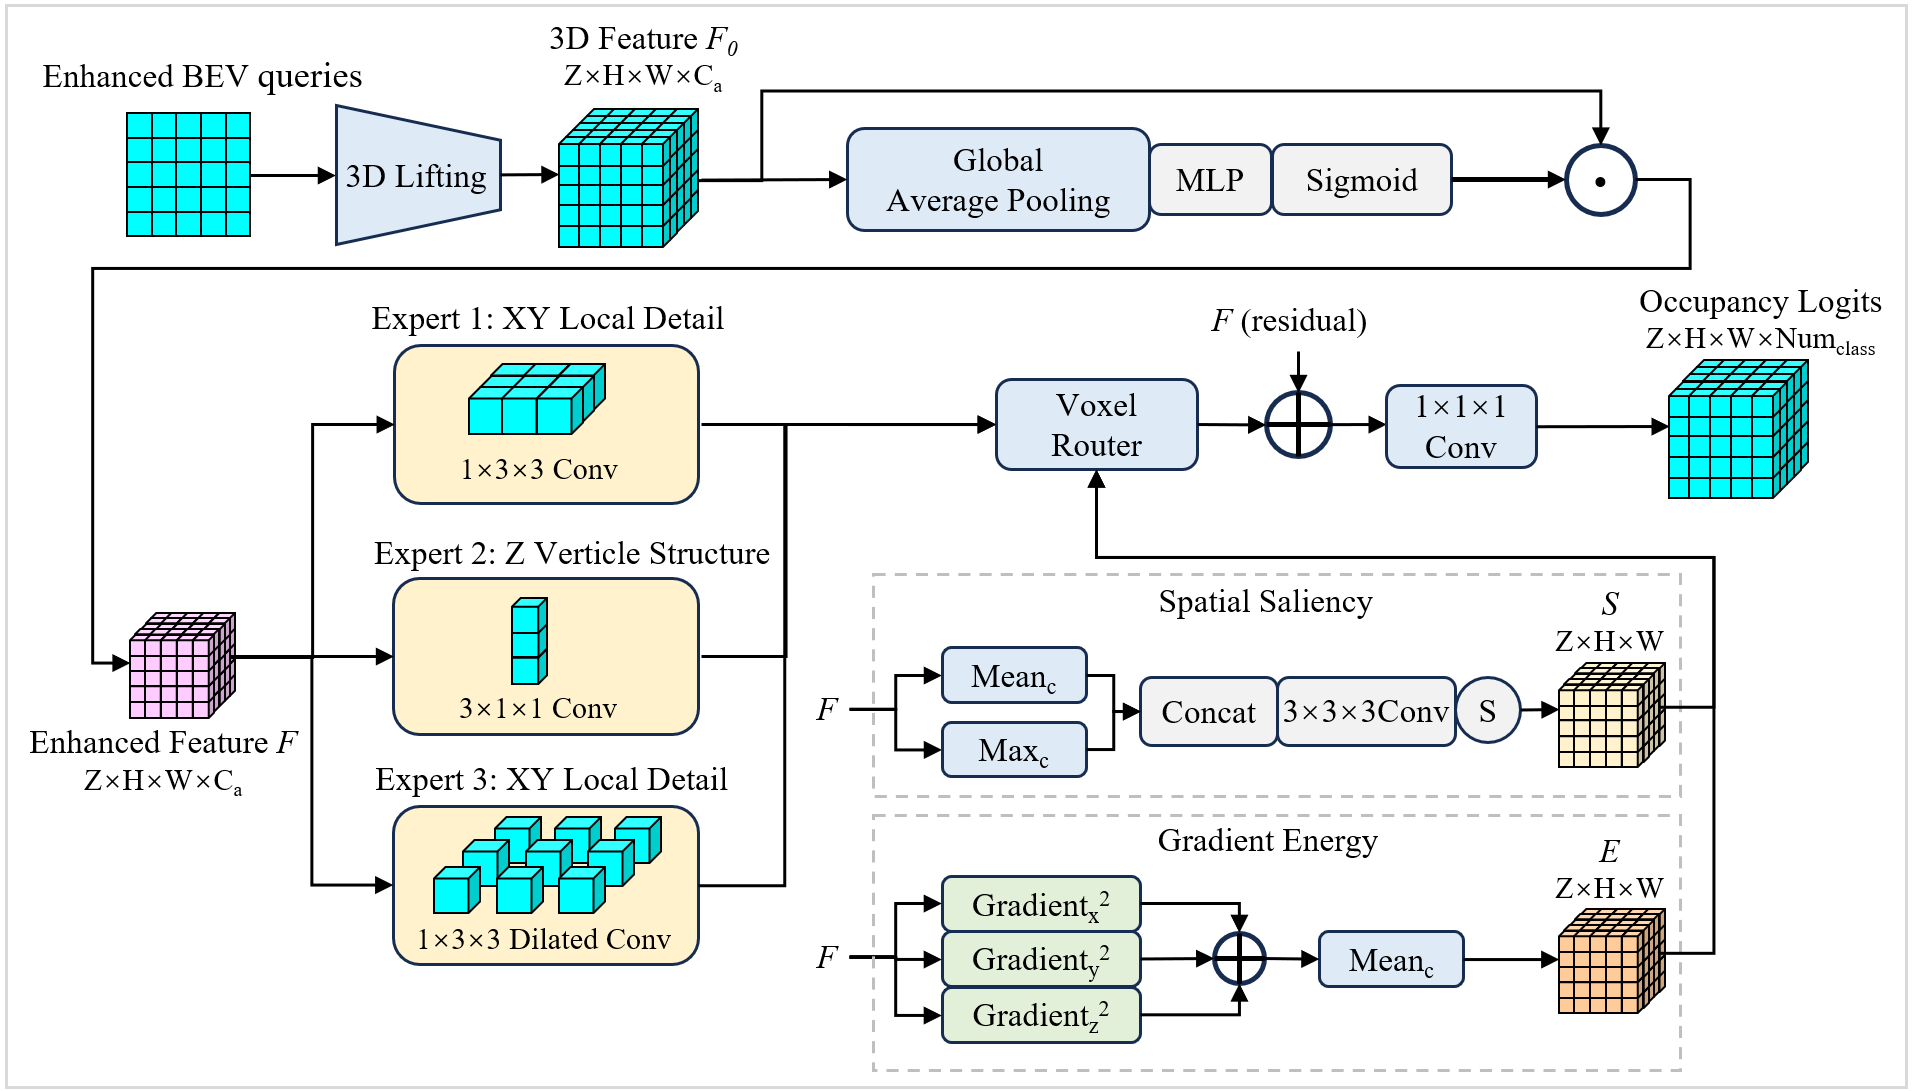
\includegraphics[width=\linewidth]{agri-amoe.png}
\caption{Agri-AMoE 三维占用解码器。二维 BEV token 经 lifting 形成三维体积，并首先由通道注意力增强；增强特征一方面并行输入三个各向异性专家，另一方面生成空间显著性与三方向梯度能量以计算逐体素路由权重。三个专家输出经加权求和与残差融合后完成最终分类。}
\label{fig:agri-amoe}
\end{figure}

\subsection{范围一致的作物感知采样}\label{sec:cropsample}
农作物的感知精度对农业机器人的田间沿行行驶非常关键。我们发现在农田场景中，土壤、道路等常见体素在样本中大量存在，而作物的体素则在不同场景中的数量差异较大。
体素中农作物占比低的样本虽包含大量地面和自由空间监督，却难以提供足够的植株边界观测，进而导致农作物感知精度的下降。
因此，本文提出一种用于训练期的数据采样策略，以小比例样本配额替换增加作物监督曝光。
对训练集第 $i$ 帧，先在预测范围内统计有效作物体素数
\begin{equation}
n_i=\sum_{v\in\V_i}\mathbf 1[y_v=\mathrm{crop}],\qquad
\mathcal D_+=\{i:n_i\ge T\}.
\end{equation}
$T$ 是含作物样本的筛选阈值；原始大范围下的作物数量不能直接用于小范围训练的样本筛选。
每个 epoch 先随机排列全部 $N$ 个训练索引，再选取 $K=\operatorname{round}(\rho N)$ 个位置，以从 $\mathcal D_+$ 中有放回均匀抽取的索引替换。
优先从 $n_i<T$ 的位置中选择替换位置；不足时扩展候选位置集合。
因此，每轮长度与基础采样一致，没有额外追加一批训练帧。
我们的模型使用 $\rho=0.10$、$T=500$。

\subsection{优化目标}\label{sec:loss}
三路当前占用输出接受相同语义真值监督。
与 SurroundOcc、OpenOccupancy 的常见体素监督一致\citep{wei2023surroundocc,wang2023openoccupancy}，每路采用类别交叉熵、语义尺度、几何尺度及 Lov\'{a}sz-Softmax 项：
\begin{equation}
\mathcal L=\sum_{j=1}^{3}\left(\lambda_{\mathrm{ce}}\mathcal L_{\mathrm{ce}}^{(j)}+
\lambda_{\mathrm{sem}}\mathcal L_{\mathrm{sem}}^{(j)}+
\lambda_{\mathrm{geo}}\mathcal L_{\mathrm{geo}}^{(j)}+
\lambda_{\mathrm{lov}}\mathcal L_{\mathrm{lov}}^{(j)}\right).
\end{equation}
$j$ 为输出分支索引；本文四个 $\lambda$ 均为 1，交叉熵内部采用 Free 为 1、其余语义类为 5 的类别权重。
所有项只作用于有效体素，地表以下的体素视为无效，不参与计算。
\section{实验}\label{sec:experiments}
\subsection{数据与评价协议}\label{sec:data}
我们在第\ref{sec:agriocc_dataset}节的所述的AgriOcc-dataset上进行了占用实验。
数据集沿x轴（前方）覆盖的空间范围为 0 m 至 15 m，沿y轴覆盖的空间范围为 −7.5 m 至 7.5 m，沿z轴覆盖的空间范围为 −2 m 至 3 m。
占用标签使用大小为0.2m*0.2m*0.2m的体素定义，共分为6个类别：Free、Crop、Soil、Drivable、Other veg.和Other obs.。
对类别 $c$，定义 $\IoU_c=\mathrm{TP}_c/(\mathrm{TP}_c+\mathrm{FP}_c+\mathrm{FN}_c)$；mIoU 为六类 IoU 的算术均值，包括 Free。
用于评价的模型取最后一个训练 epoch。
另以 ORAD-3D 官方测试集及其农田子集评价真实环境的迁移效果，并在独立采集的高分辨率仿真数据上评价体素分辨率迁移的迁移效果。

\subsection{实现细节}\label{sec:implementation}
模型的图像编码器采用ResNet-101--FPN，使用预训练权重初始化。
输入图像为 $512\times288$，BEV 查询为 $75\times75$，通道数 256，编码器 6 层，Agri-AMoE 宽度 96。
AdamW 初始学习率为 $2\times10^{-4}$，权重衰减为 0.01；采用余弦衰减与 500 次迭代线性 warm-up。
在3张RTX 4090显卡上训练 15 个 epoch，全局 batch size 为 24。CropSample 主配置为 $\rho=0.10,T=500$。
训练集 32,385 帧中有 20,300 帧达到这一作物阈值，每轮最多替换约 3,238 个位置。
各对比方法使用其原有模型架构与优化目标；共用预测范围、三路前视输入、图像尺寸、数据划分和训练轮数。

\subsection{与现有方法比较}\label{sec:comparison}
表\ref{tab:main}给出AgriOcc与几种先进语义占用方法的对比结果。
SurroundOcc\citep{wei2023surroundocc}、SparseOcc\citep{tang2024sparseocc}与 COTR\citep{ma2024cotr}同属当前帧语义占用方法；
Drive-OccWorld\citep{yangDrivingOccupancyWorld2025}和 IR-WM\citep{mei2025irwm}则同时预测当前与未来占用。
我们保留它们的历史输入、未来占用和轨迹联合任务，仅比较其当前帧输出。
结果表明，AgriOcc 在各类别的IoU上均优于各对比方法。

\begin{table}[pos=htbp]
\centering
\caption{AgriOcc-Dataset上的三维语义占用性能（\%）。}
\label{tab:main}
\resizebox{\linewidth}{!}{%
\begin{tabular}{lrrrrrrrr}
\toprule
方法 & 参数(M) & mIoU & Free & Crop & Soil & Drivable & Other veg. & Other obs.\\
\midrule
SurroundOcc & 198.24 & 61.84 & 93.43 & 30.67 & 80.46 & 73.05 & 49.73 & 43.72 \\
SparseOcc & 58.14 & 33.35 & 89.24 & 6.95 & 45.14 & 36.88 & 9.96 & 11.95 \\
COTR & 37.16 & 56.24 & 89.86 & 26.65 & 76.56 & 61.47 & 46.91 & 35.98 \\
Drive-OccWorld & 60.68 & 35.15 & 85.52 & 19.63 & 40.29 & 29.64 & 21.06 & 14.77 \\
IR-WM & 58.42 & 38.62 & 86.93 & 21.20 & 46.68 & 33.01 & 24.68 & 19.25 \\
AgriOcc & 53.03 & 64.08 & 93.55 & 39.38 & 80.57 & 74.38 & 50.69 & 45.91 \\
\bottomrule
\end{tabular}}
\end{table}

AgriOcc 达到 64.08\% mIoU，较 SurroundOcc 的 61.84\% 增加 2.24 个百分点，相对提高 3.6\%。
作物 IoU 由 30.67\% 增至 39.38\%，提高 8.71 个百分点；土壤与可通行区域分别达到 80.57\% 和 74.38\%。
相比之下，IR-WM 与Drive-OccWorld的结果还受到未来预测与规划联合目标的影响，因此在三维语义占用的性能上没有优势。
SurroundOcc、SparseOcc 和 COTR 的设计主要面向城市环视驾驶场景：
均匀的空间查询与城市道路先验难以直接适配农业机器人前方视域中的行间遮挡、细长作物和近场精细边界。
相比之下，IR-WM 与 Drive-OccWorld 的重点是利用历史状态、动作条件和未来滚动预测服务于世界建模与规划；
在当前帧占用预测的任务下，这些额外能力无法充分转化为当前体素精度，且多步联合优化会增加表征学习的难度。因此，它们较低的当前帧指标反映了任务目标与模型归纳偏置的不匹配，而非世界模型在预测未来状态或规划任务中的能力不足。

图\ref{fig:comparison}和图\ref{fig:comparison_sparse}在三个相同场景上比较预测。
各方法使用同一真值有效性掩码与语义配色；视角固定于移动平台正后上方，沿前进方向观察。
AgriOcc 能恢复主要地面布局与植被区域，相比于其他方法，能有效改进作物分析效果。
\begin{figure}[pos=htbp]
\centering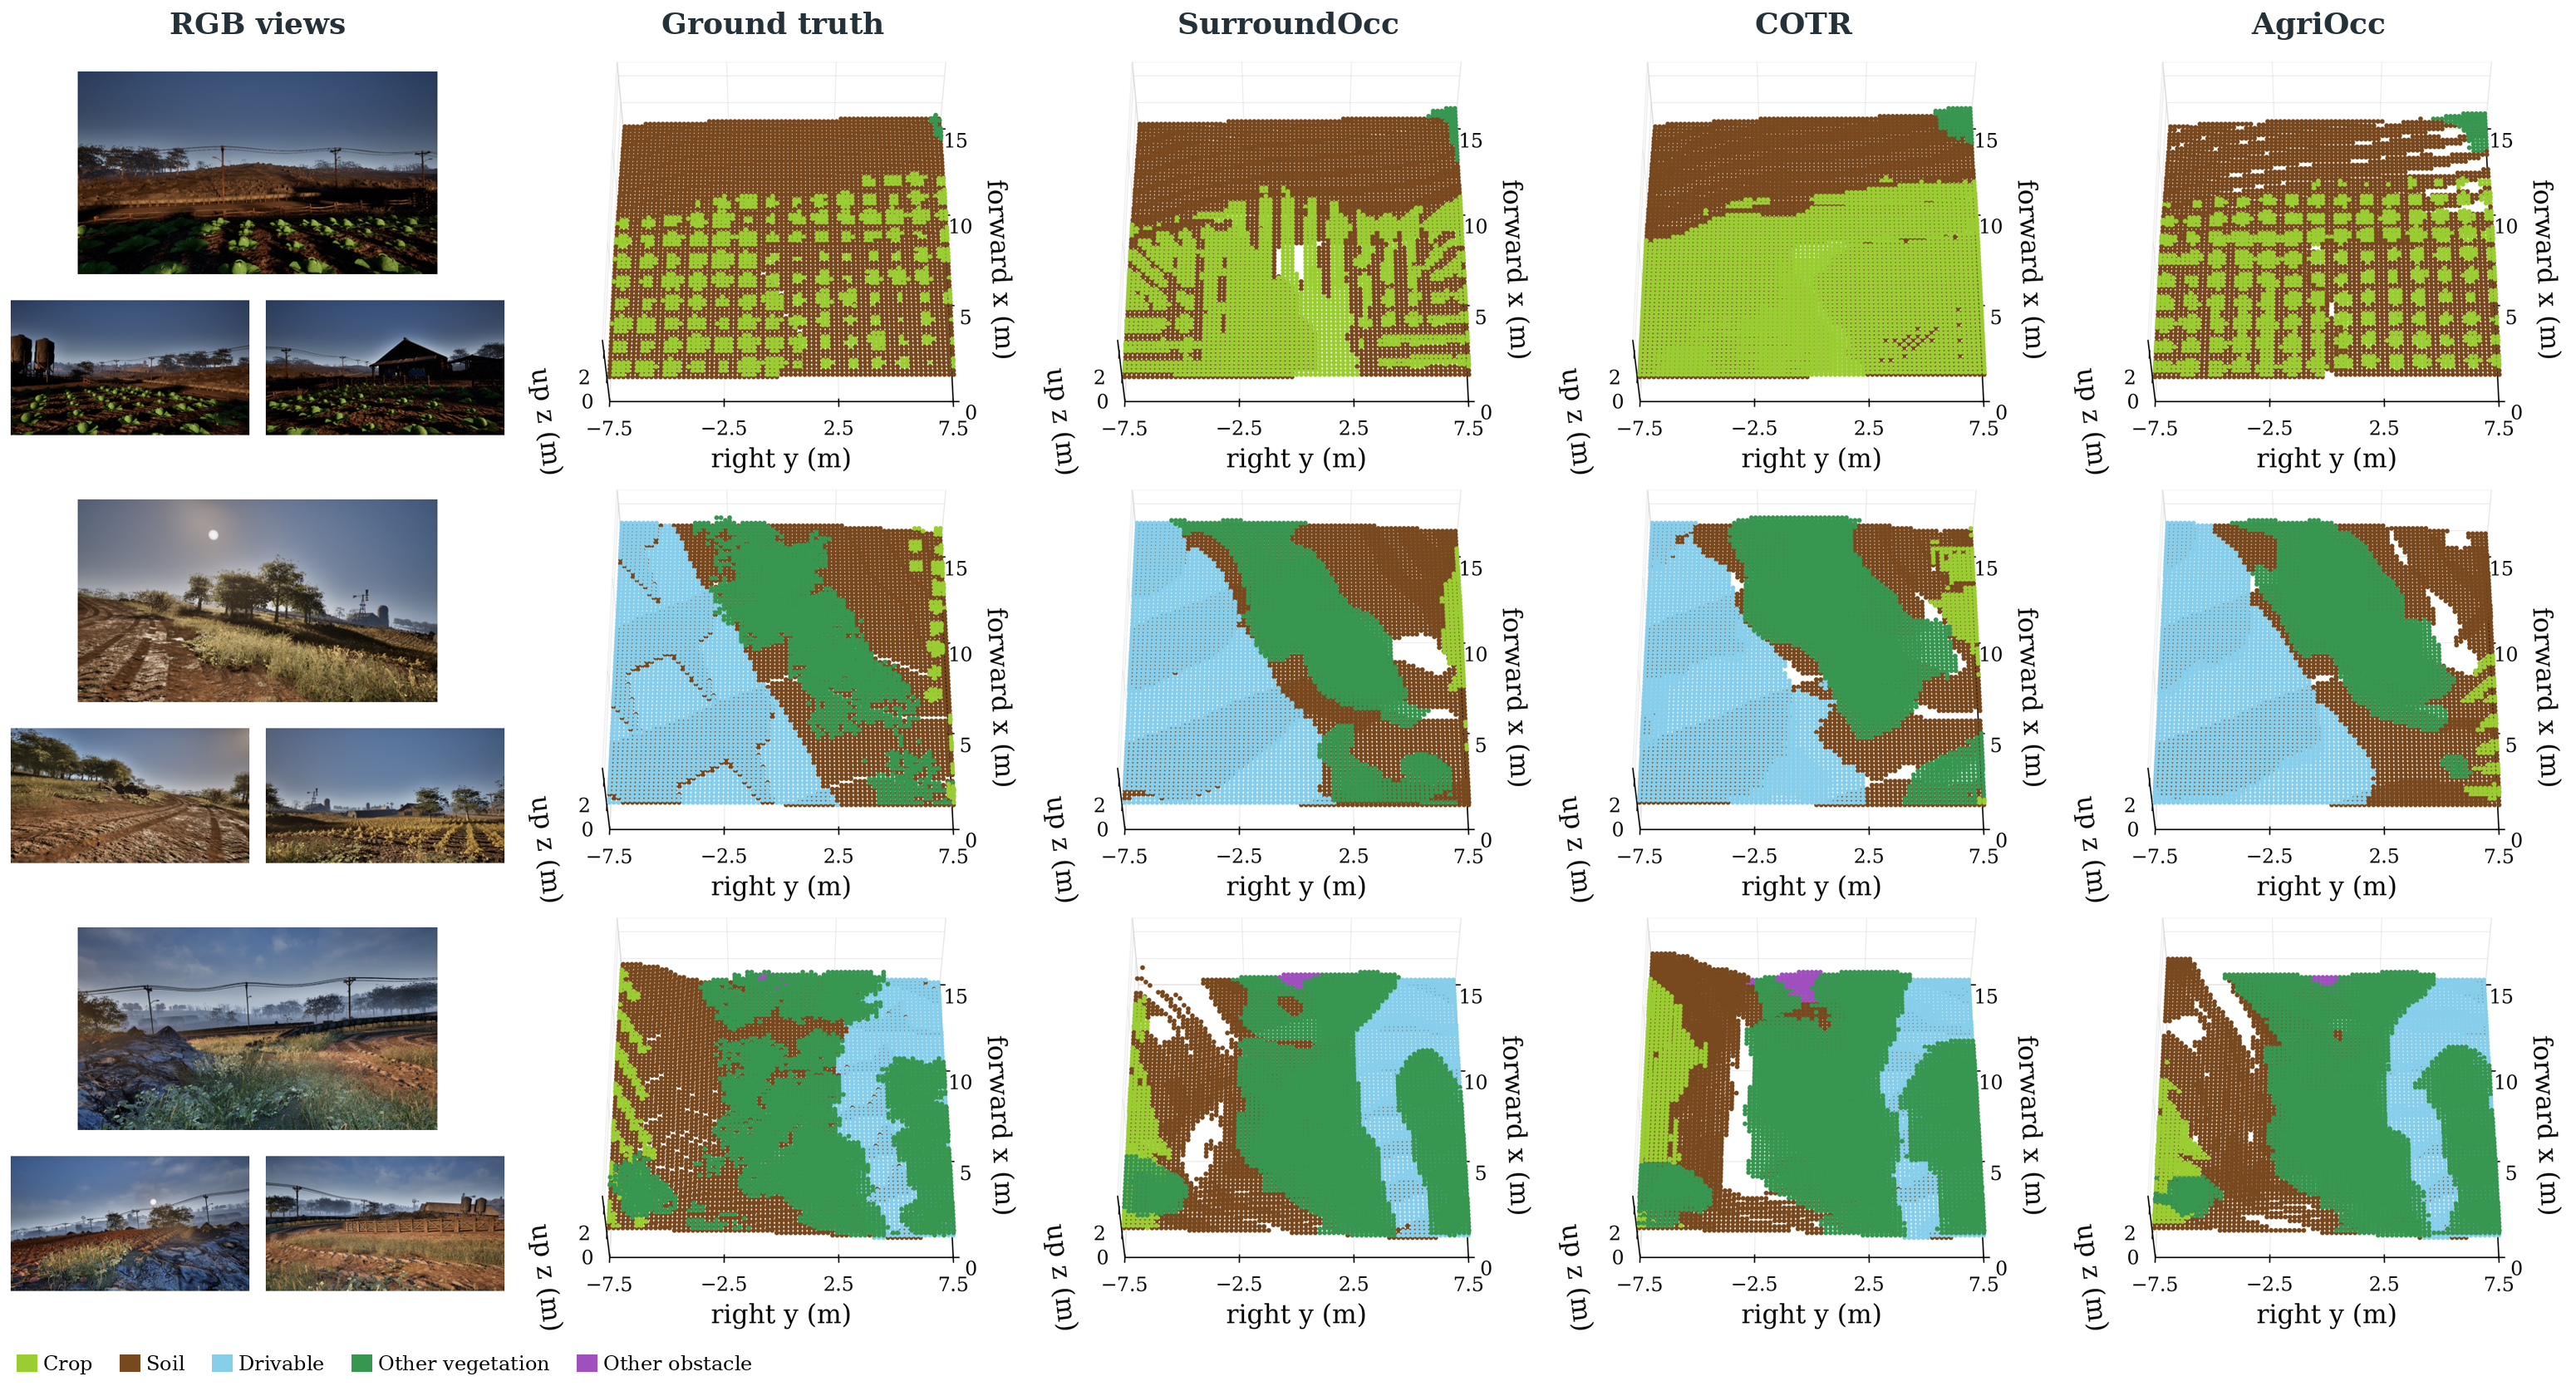
\includegraphics[width=\linewidth]{qualitative_comparison.png}
\caption{当前帧占用定性比较。从左至右为三路 RGB、GT、SurroundOcc、COTR与 AgriOcc。各占用效果图采用相同的正后上方视角、范围与有效体素掩码。}
\label{fig:comparison}
\end{figure}
\begin{figure}[pos=htbp]
\centering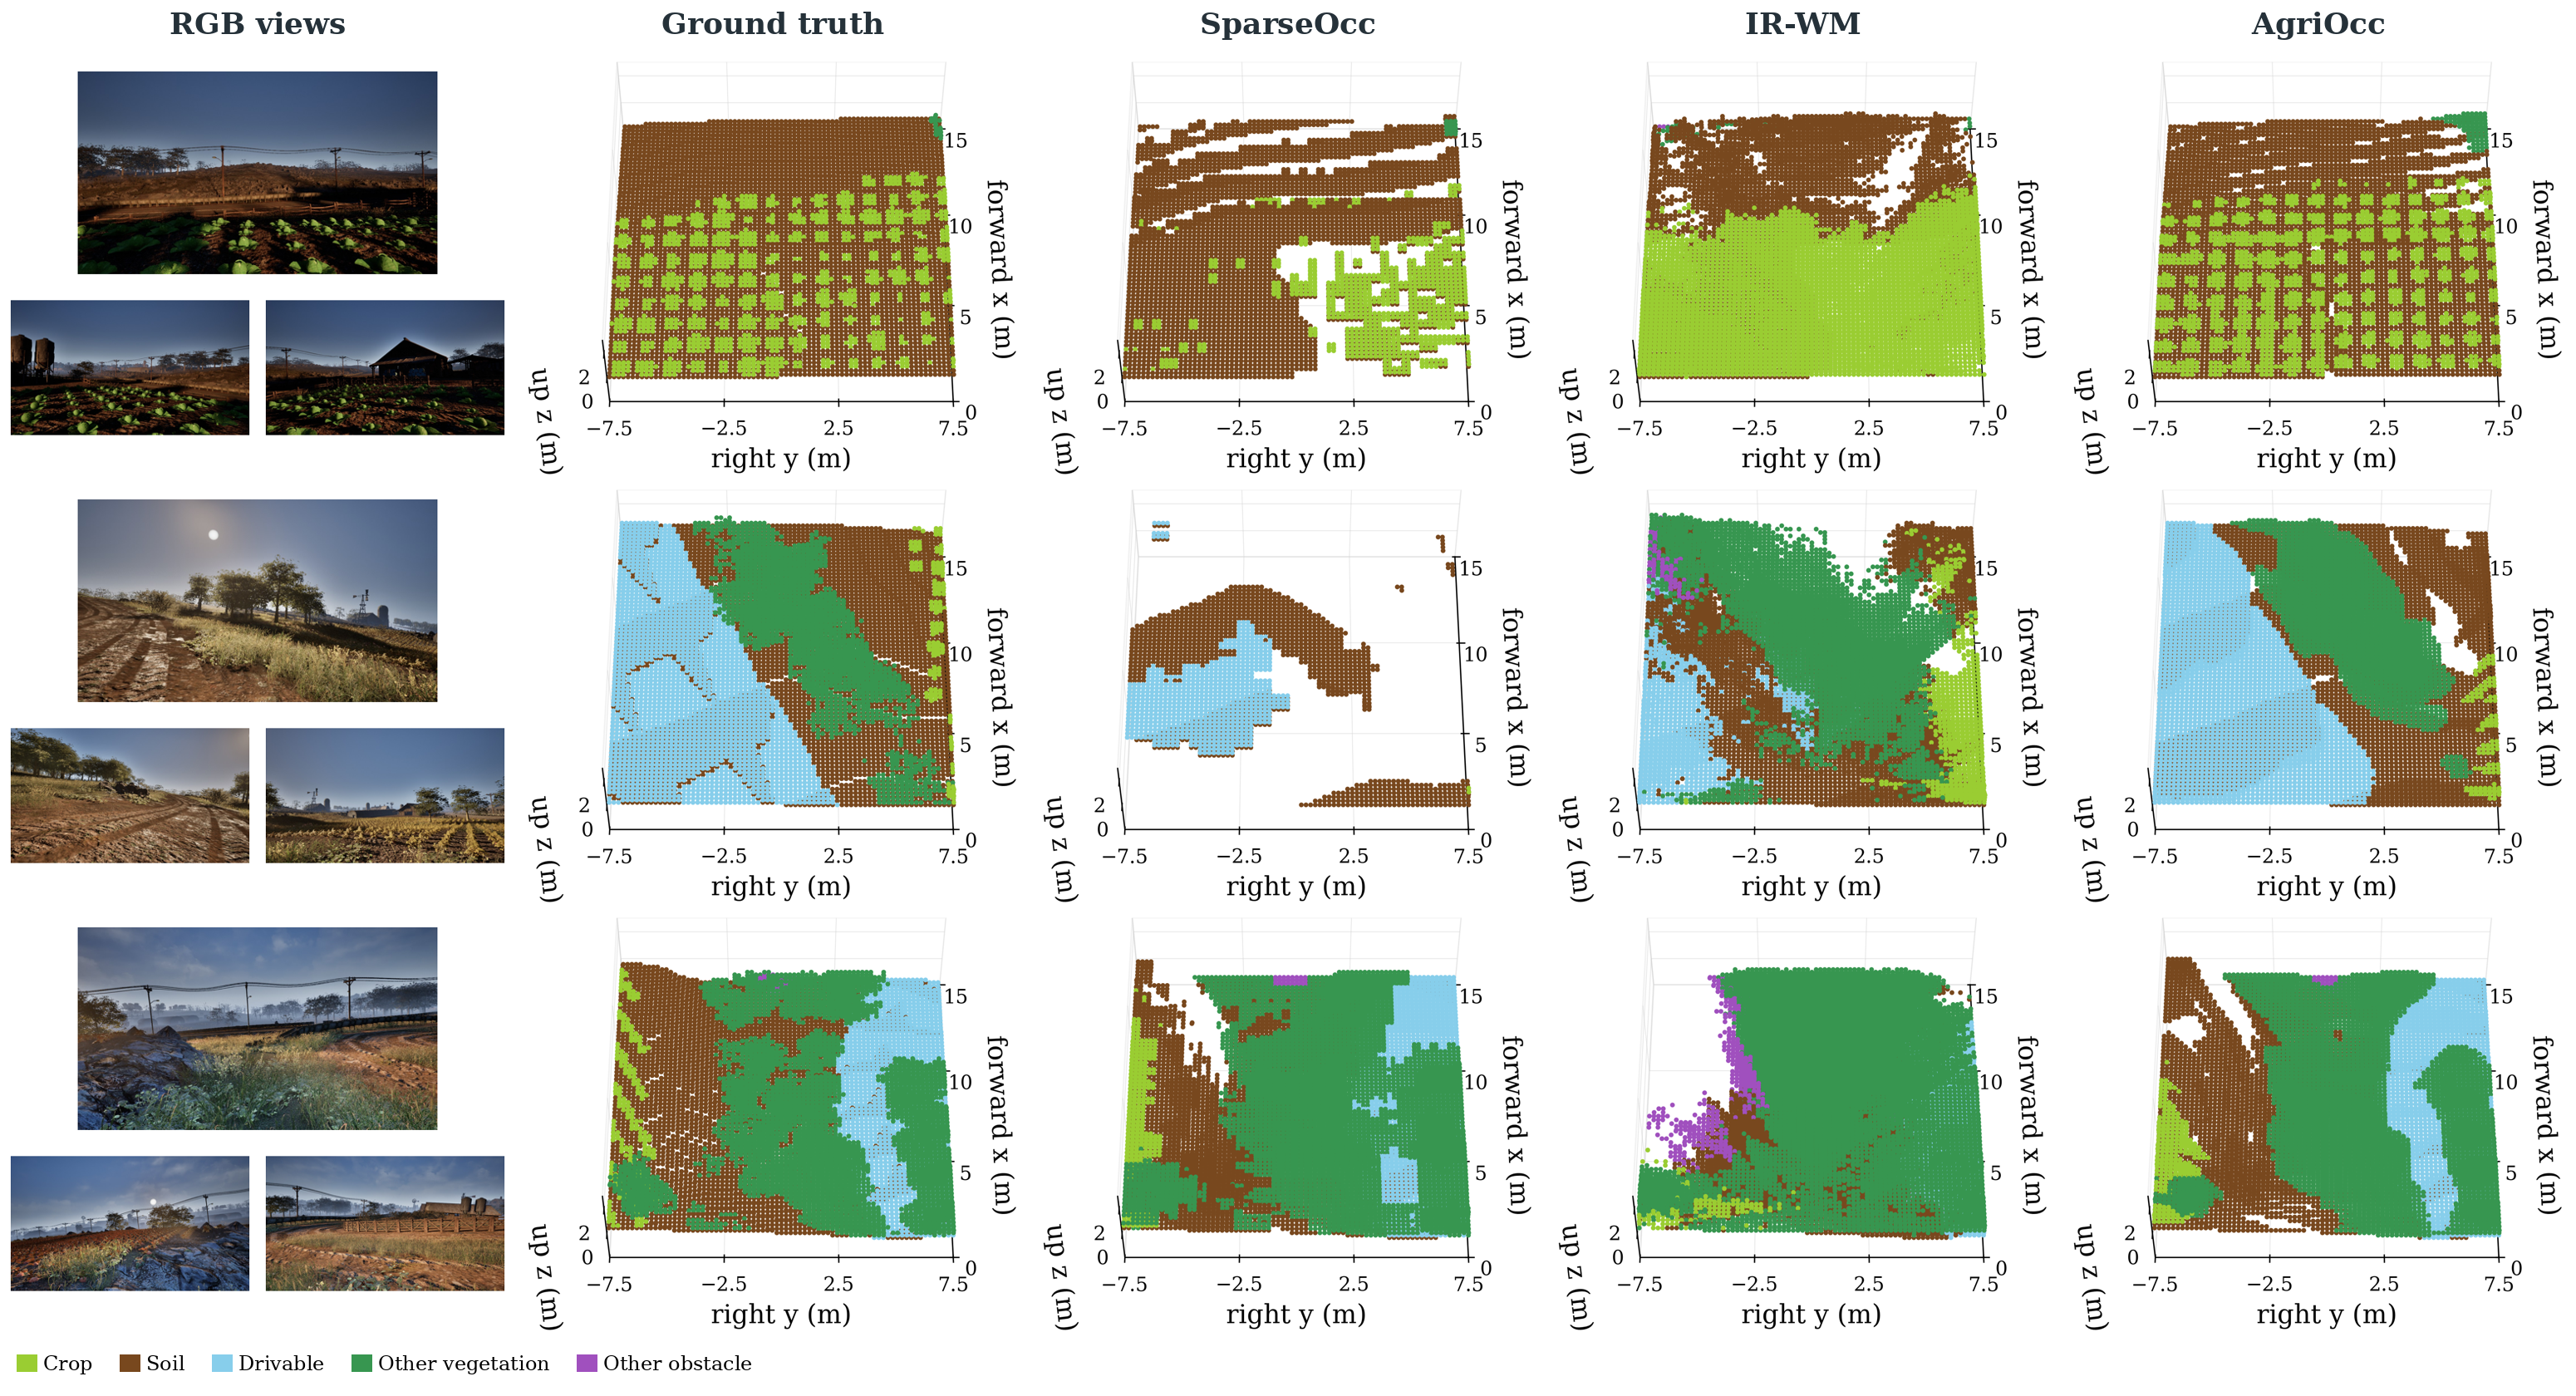
\includegraphics[width=\linewidth]{qualitative_sparse_irwm.png}
\caption{与 SparseOcc和IR-WM 定性比较，列顺序为 RGB、GT、SparseOcc、IR-WM 与 AgriOcc。采用与图\ref{fig:comparison}一致的视角和语义颜色。}
\label{fig:comparison_sparse}
\end{figure}

\subsection{结构与训练策略消融}\label{sec:ablation}

\paragraph{模型主要组件消融}
表\ref{tab:ablation}分别比较基础网络、Agri-AMoE 以及加入 CropSample 的最终模型。
所有配置共享相同的图像编码器和BEV编码器，仅改变解码器和训练采样策略。
仅加入 Agri-AMoE，mIoU 从 63.76\% 提升至 64.20\%，作物 IoU 从 37.76\% 提升至 38.93\%。
进一步使用 CropSample 后，作物 IoU 提升到 39.38\%，但 mIoU 略降至 64.08\%。

\begin{table}[pos=htbp]
\centering
\caption{消融实验。}
\label{tab:ablation}
\begin{tabular}{lrrrr}
\toprule
配置 & 采样 $(\rho,T)$ & 可训练参数(M) & mIoU(\%) & Crop IoU(\%)\\
\midrule
Base & -- & 52.37 & 63.76 & 37.76\\
Base + Agri-AMoE & -- & 53.03 & 64.20 & 38.93\\
AgriOcc & $(0.10,500)$ & 53.03 & 64.08 & 39.38\\
\bottomrule
\end{tabular}
\end{table}

\paragraph{Agri-AMoE消融}


\paragraph{采样策略消融}
在试验中我们发现，提高作物样本曝光并不必然提高所有类别的 IoU。
表\ref{tab:sampling}给出了我们在不同采样设置下的试验结果。
试验所用模型架构为Base+AgriAMoE，固定 $T=500$ 时，$\rho=0.10$ 到 $0.20$ 的作物 IoU 仅从 39.38\% 增至 39.46\%，mIoU 却降至 63.23\%。
较高配额会压缩部分背景样本的曝光，并改变模型的类别决策平衡；因此本文采用比较均衡的 $0.10$ 阈值。

\begin{table}[pos=htbp]
\centering
\caption{采样敏感性结果。}
\label{tab:sampling}
\begin{tabular}{lrrr}
\toprule
模型 & $(\rho,T)$ & mIoU(\%) & Crop IoU(\%)\\
\midrule
Base + Agri-AMoE & 无采样 & 64.20 & 38.93\\
Base + Agri-AMoE & $(0.10,500)$ & 64.08 & 39.38\\
Base + Agri-AMoE & $(0.15,500)$ & 63.67 & 39.02\\
Base + Agri-AMoE & $(0.20,500)$ & 63.23 & 39.46\\
\bottomrule
\end{tabular}
\end{table}



\subsection{真实场景迁移与定性分析}\label{sec:sim2real}
\subsubsection{仿真到真实数据集的迁移}\label{sec:orad_transfer}
为了进一步验证仿真数据集上训练的模型在真实世界的有效性，本节我们在 ORAD-3D 数据集\citep{chen2025orad3d}上
对 AgriOcc-Dataset 上训练好的模型进行迁移学习，并评估其官方测试集和农田子集上的性能。
ORAD-3D 的占用预测网格形状为 $100\times100\times16$，共有九类体素，类别定义沿用其官方标注协议。
AgriOcc 的输入接口按三路前视相机设计，与 ORAD-3D 提供的环视传感器配置不匹配，
且两者的类别体系也不相同，因此本文只取中心前视相机的 BEV embedding，
替换为适配目标网格形状与类别数的占用头，再使用 ORAD-3D 训练集进行对齐训练。

我们使用在 AgriOcc-Dataset 上预训练的模型进行目标域适配，并与从头训练的 AgriOcc 模型和 ORAD-3D 论文中的基准模型进行比较。
表\ref{tab:orad}同时给出 ORAD-3D 官方测试集和从中筛选出的农田场景子集的结果。
\texttt{Test} 在完整类别上计算，\texttt{Test\_farm} 则按农田子集中出现的类别计算。
为与 ORAD-3D 论文中的语义 mIoU 保持可比，表中额外报告去除 Free 类后的 Test mIoU。
表中OpenOcc、OccFormer 和 SurroundOcc 的结果引自 ORAD-3D 论文\citep{chen2025orad3d}。
结果表明，在相同的完整目标域训练数据下，AgriOcc-Dataset 预训练后仅需 2 个 epoch 的适配，
即可在 \texttt{Test (w/o Free)} 上达到 11.17\%，高于从头训练的 9.01\% 与 ORAD-3D 论文中报告的 7.60\%，
同时将目标域训练时间由 54.1 分钟降至 18.5 分钟。
这说明仿真农业数据预训练获得的图像--BEV 几何与三维语义先验能够有效迁移到真实越野场景，
从而以更低的目标域适配成本提升语义占用预测性能。

 
表\ref{tab:orad}使用独立测试集结果。
Test 为固定九类平均，Test w/o Free 为去掉 Free 的八类平均；Farm 也使用九类。
\begin{table}[pos=htbp]
\centering
\caption{ORAD-3D 仿真到真实迁移结果（\%）。两组 AgriOcc 均使用完整 ORAD-3D 训练集，
并仅使用中心前视相机输入；迁移模型以 AgriOcc-Dataset 预训练权重初始化后进行 2 个 epoch 适配。
\texttt{Test (w/o Free)} 为去除 Free 类别后的 mIoU，与 ORAD-3D 论文口径一致；
\texttt{Test} 为全部九类的 mIoU；\texttt{Test\_farm} 为农田场景子集上按出现类别计算的 mIoU。
OpenOcc、OccFormer 与 SurroundOcc 的结果引自 ORAD-3D 论文.}
\label{tab:orad}
\fontsize{9}{11}\selectfont
\setlength{\tabcolsep}{2.6pt}
\begin{tabular}{lrrrr}
\toprule 
方法 & 训练时间(min) & Test (w/o Free) & Test & Test\_farm \\
\midrule
OpenOcc\citep{jiang2024openocc} & -- & 5.83 & -- & -- \\
OccFormer\citep{zhang2023occformer} & -- & 7.45 & -- & -- \\
SurroundOcc\citep{wei2023surroundocc} & -- & 7.60 & -- & -- \\
\midrule
AgriOcc（从头训练） & 54.1 & 9.01 & 18.16 & 31.83 \\
\midrule
AgriOcc（预训练迁移） & 18.5 & \textbf{11.17} & \textbf{20.11} & 39.45 \\
\bottomrule
\end{tabular}
\end{table}

两轮迁移将目标域训练时间减少 66.7\%，但完整测试集 mIoU 比六轮从头训练低 0.89 个百分点；固定口径的 Farm mIoU 相差约 0.10 个百分点。
该结果表明，源域占用表征能够在较短适配预算下获得接近的农田子集表现，同时仍存在全测试集精度差距。
两个设置训练预算不同，不能据此断言同等训练轮数下迁移的优劣。
图\ref{fig:orad}展示同一批真实农田测试帧，两组预测都呈现出主要道路布局，但局部占用边界及细小、稀有类别的识别仍具有挑战。
\begin{figure}[pos=htbp]
\centering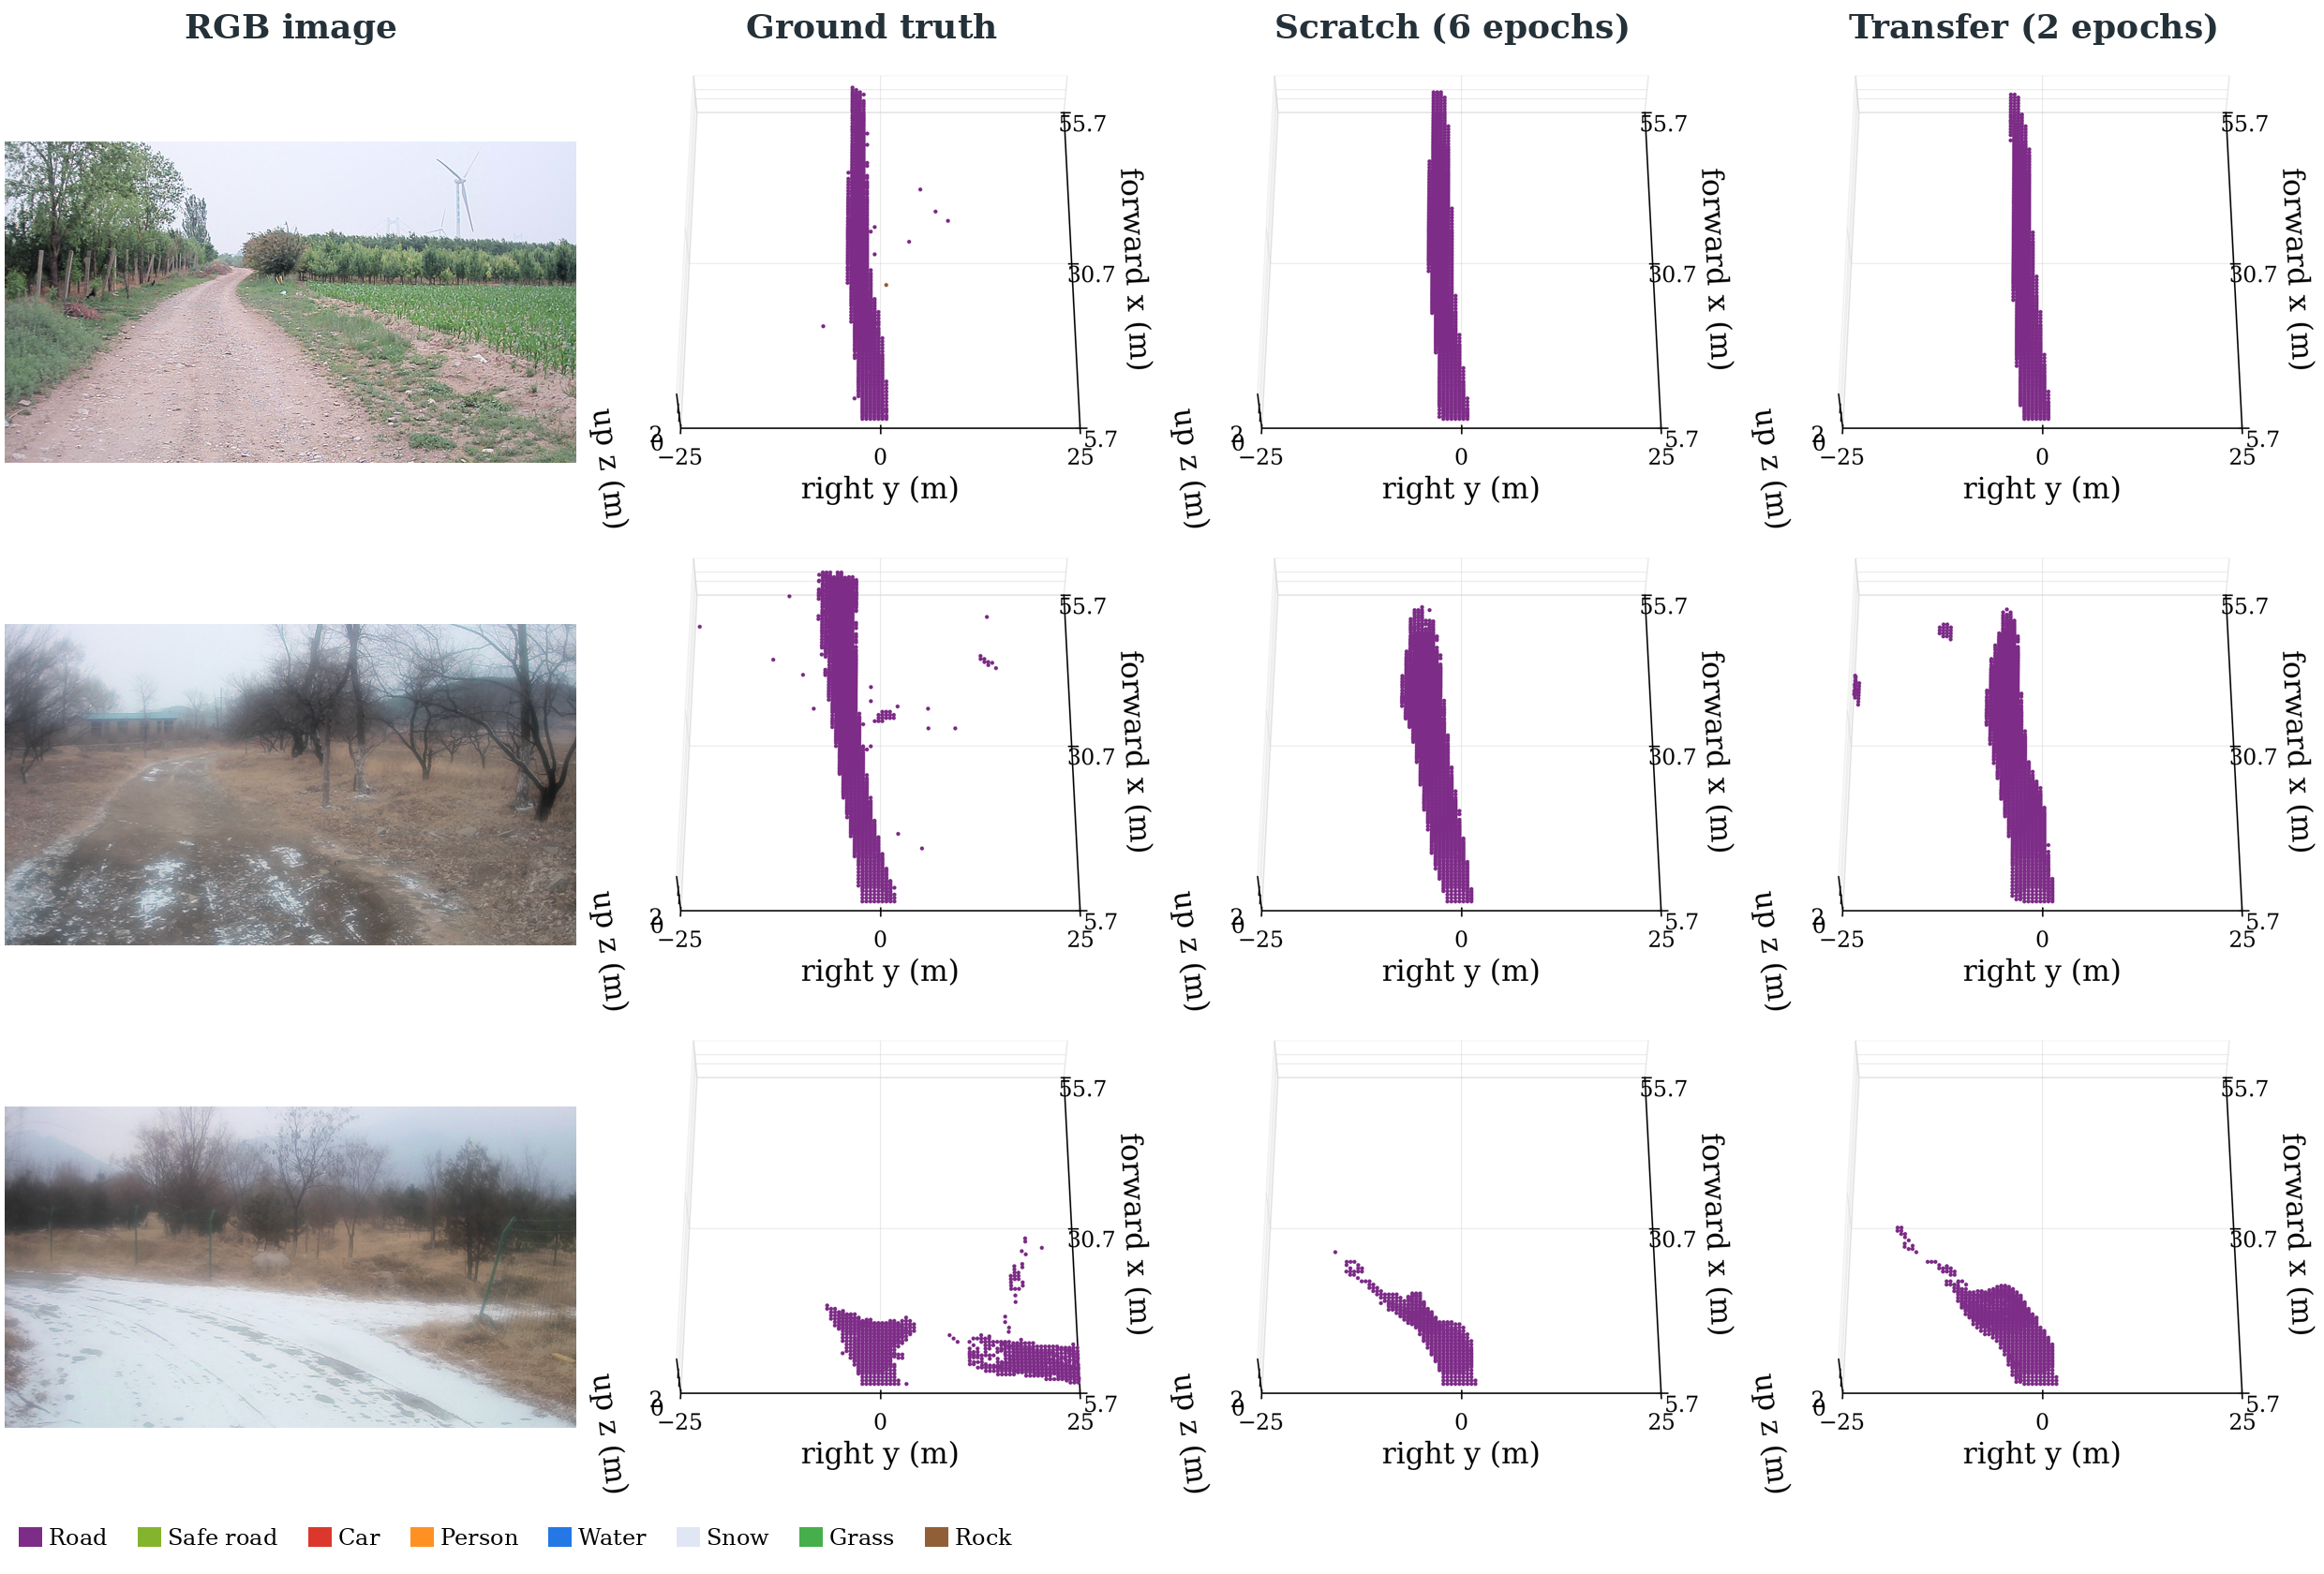
\includegraphics[width=\linewidth]{orad_transfer.png}
\caption{ORAD-3D 定性迁移结果。列顺序为单目 RGB、GT、6 轮从头训练与 2 轮源域迁移。两模型均使用目标域官方网格，采用相同正后上方视角与 GT 有效掩码；自由空间不显示。}
\label{fig:orad}
\end{figure}

\subsubsection{真实农田 Zero-shot 定性分析}\label{sec:realfield_zeroshot}
除 ORAD-3D 的迁移实验外，我们进一步在哈尔滨工业大学智慧农场验证中心采集真实的大豆田图像，来定性分析AgriOcc在真实农田场景的性能。、
4组例图的预测结果见图\ref{fig:realfield_zeroshot}。
四个场景包含两处田块的作物垄行和耕作前裸土：它们在作物密度、土壤纹理、背景建筑、树木遮挡和光照条件上均与 AgriOcc-Dataset 存在明显差异。
我们直接采用 AgriOcc-Dataset 上训练的AgriOcc进行Zero-shot推理，未使用真实农田数据进行微调。

在两组作物垄行场景中，预测结果均恢复了作物与土壤地面交替的长条带结构，且在 $20\,$m 前向范围内保持了垄行的方向连续性。
对于两组裸土场景，模型将绝大多数近地体素判定为 soil\_ground，并保留由耕作纹理形成的前向结构；远处树木和建筑附近仍会产生少量其他植被、障碍物或可通行区域的预测结果。
这些结果表明，AgriOcc 从仿真农田中学习到的图像--BEV 几何布局和作物--土壤结构先验能够在未见真实田块中形成合理的三维语义占用布局。
由于该组实验不含同步采集的体素真值，我们将其作为 zero-shot 可视化分析，进一步验证了我们利用仿真数据训练的AgriOcc在真实农田场景的同样具备有效的空间理解能力。

\begin{figure}[pos=htbp]
\centering
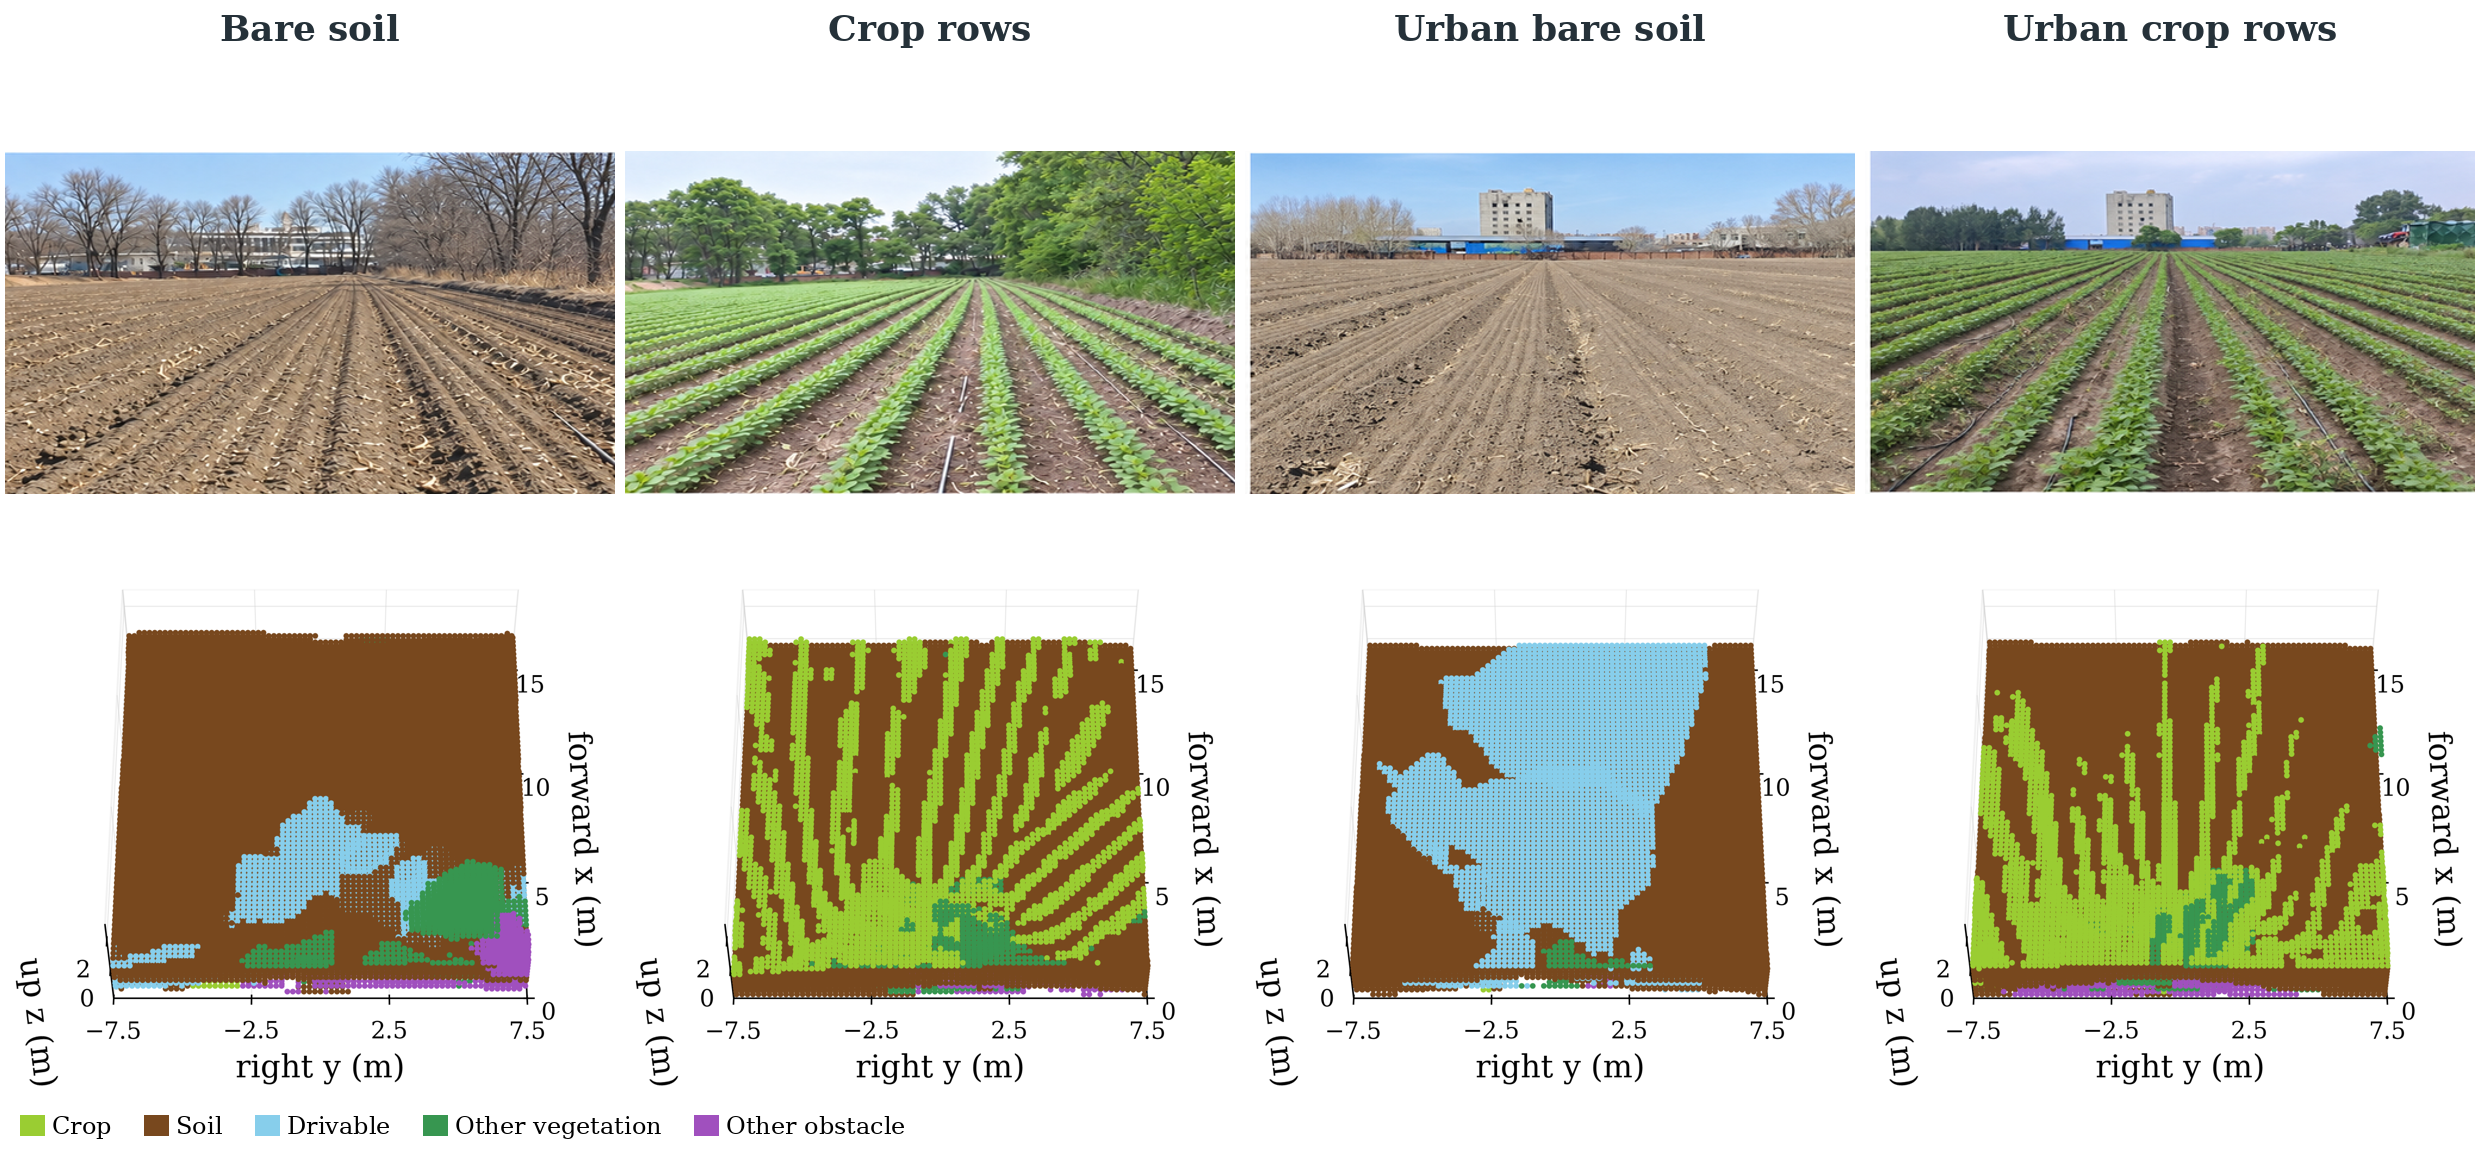
\includegraphics[width=\linewidth]{realfield.png}
\caption{真实农田 zero-shot 三维语义占用预测。}
\label{fig:realfield_zeroshot}
\end{figure}


\subsection{体素分辨率迁移}\label{sec:resolution}
本文构建的 AgriOcc-Dataset 的体素分辨率为 $0.2\,\mathrm{m}$，与主流自动驾驶语义占用基准一致\citep{behley2019semantickitti,li2024sscbench}。
但是农业机器人在垄间通行、株间避障和精细作业时，$0.2\times0.2\times0.2\,\mathrm{m}$ 的体素可能将相邻作物、
窄垄沟或局部可通行边界量化到同一网格中，带来潜在的精度不足问题。
然而，将整个 BEV 编码器直接扩展到 $0.1\times0.1\times0.2\,\mathrm{m}$ 会使
XY 查询数从 $75\times75$ 增至 $150\times150$，即增加四倍；
相应地，多尺度图像--BEV 交互、BEV 中间激活和三维占用监督的计算与显存开销均显著上升。
为此，我们另外采集了一个 $0.1\times0.1\times0.2\,\mathrm{m}$ 分辨率的小型仿真数据集，
包含 19,300 个样本，并按 1:1 划分为训练集和验证集。
我们使用它来进一步验证 AgriOcc 是否能够将已学习的标准分辨率三维先验高效迁移到细分辨率占用预测。

具体地，迁移模型首先在 $0.2\times0.2\times0.2\,\mathrm{m}$ 的 AgriOcc-Dataset 上完成训练。
在 $0.1\times0.1\times0.2\,\mathrm{m}$ 数据上，我们比较两种冻结主干的适配方式：
\emph{查询适配}保留主干参数，仅学习 $150\times150$ 高分辨率 BEV 查询格点；
\emph{细化头适配}保留原有 $75\times75$ BEV 编码器与 Agri-AMoE 解码器，冻结其全部已有权重，
仅在占用输出端训练学习式 $2\times$ 细化头。该头将粗占用 logits 与对应的 BEV 特征投影融合，
输出 $150\times150\times25$ 体素。对照组不使用 $0.2\,\mathrm{m}$ 占用预训练权重，
而是在同一个 $0.1\,\mathrm{m}$ 数据集上从头学习 $150\times150$ 的高分辨率 BEV 与占用预测；
三组均在同一小范围、高分辨率标签上训练 15 轮。实测结果见表\ref{tab:resolution}。
\begin{table}[pos=htbp]
\centering
\caption{体素分辨率迁移，IoU 单位为\%，时间为 15 轮目标分辨率训练与逐轮验证的日志墙钟小时数，不包含 $0.2\,\mathrm{m}$ 源训练。所有行均输出 $150\times150\times25$。}
\label{tab:resolution}
\resizebox{\linewidth}{!}{%
\begin{tabular}{lrrrrrrrr}
\toprule
设置 & 时间(h) & mIoU & Free & Crop & Soil & Drivable & Other veg. & Other obs.\\
\midrule
0.1 m 从头训练 & 15.47 & 46.55 & 92.27 & 22.42 & 66.66 & 39.51 & 33.44 & 25.00 \\
查询适配（冻结主干） & 11.40 & 45.34 & 91.67 & 22.43 & 64.72 & 30.70 & 34.82 & 27.71 \\
细化头适配（冻结主干） & 4.72 & 49.67 & 92.70 & 29.10 & 71.72 & 38.51 & 36.84 & 29.14 \\
\bottomrule
\end{tabular}}
\end{table}

表\ref{tab:resolution}显示，相比不使用 $0.2\,\mathrm{m}$ 占用预训练的从头训练，
细化头适配的 mIoU 为 49.67\%，高于从头训练的 46.55\%，提高 3.12 个百分点；作物 IoU 从 22.42\% 提高到 29.10\%。
训练时间由 15.47 小时降至 4.72 小时，减少 69.5\%。它在六个语义类别上也均取得最佳 IoU。
查询适配虽缩短时间至 11.40 小时，但 mIoU 为 45.34\%，没有超过从头训练。
这是因为细化头复用低分辨率网络已建立的场景布局与语义关系，将有限目标数据用于学习输出端的局部残差；
查询适配则改变全部 BEV 查询的空间采样密度，在冻结主干下仍需重新协调细网格表征。
细化头适配保持 $75\times75$ 编码器的稳定全局上下文，仅以 11,238 个可训练参数学习从 0.2 m 粗预测到 0.1 m 体素的高频残差。
因此，高分辨率监督能够集中恢复株间边界、垄沟与局部可通行区域，而无需重新学习相机投影关系和场景级语义布局。
上述结果表明，利用冻结主干与轻量细化头，可以将 $0.2\,\mathrm{m}$ 数据上训练的 AgriOcc 有效迁移至更高分辨率的占用预测，
并同时获得优于从头训练的精度和显著更短的适配时间。

\subsection{讨论与局限}\label{sec:discussion}
我们所提出的语义占用预测模型，具备周围空间结构的感知能力，可以有效感知农业场景中的常见要素，
可用于农业移动平台的道路识别、作物行线识别、障碍物感知与避障等应用。
然而目前本工作仅进行语义级的预测，缺乏实例级的感知。
对于动态的障碍物（如行驶中的车辆、移动的农机或动物）无法判断某个体素块所属的物体实例。
如果需要依据周围物体的运动趋势进行局部路径规划，则还需要额外部署目标检测模型。
因此AgriOcc更适用于活动物体较少的农业场景。
未来我们也将进一步研究面向农业移动平台的全景实例级语义占用，
提升农业移动平台在复杂环境下的感知能力。


\section{结论与展望}\label{sec:conclusion}
本文围绕农业机器人的前向作业视野，提出三相机当前帧语义占用框架 AgriOcc，并构建覆盖十种作物、多生长期、时段与天气的仿真数据集。
AgriOcc 保留BEVFormer的可变形 BEV 聚合架构，以 Agri-AMoE 适应地面、植株高度与局部上下文的各向异性，再通过 CropSample 在固定训练长度内增加作物监督曝光。
在前方 $15\times15\times5\,\mathrm{m}$ 的预测范围下，模型达到 64.08\% mIoU 和 39.38\% 作物 IoU。
消融揭示，结构自适应解码与作物样本曝光具有不同作用：前者改善基础表征，后者进一步调整作物与背景的决策平衡。
分辨率迁移表明，保留稳定的粗尺度模型、仅训练轻量细化头，可将 $0.2\,\mathrm{m}$ 占用先验迁移到 $0.1\times0.1\times0.2\,\mathrm{m}$ 输出，在提高精度的同时减少目标分辨率阶段训练时间。
真实环境迁移实验则说明在仿真数据上的训练的AgriOcc可以学习到真实世界的环境特征。
未来将进一步面向真实农田的光照、天气、作物生长期与传感器扰动构建更丰富的跨域训练策略；研究面向农业移动平台的全景实例级语义占用，
提升农业场景下的动态感知能力；并将 AgriOcc 的占用表征与风险感知通行性分析、轨迹优化和闭环导航深度耦合。
最终，语义占用有望成为连接各类农业移动平台感知、决策与控制的稳定三维基础模型接口。

\section*{数据与代码可得性}
AgriOcc-Dataset 的构建流程、类别定义与标注生成方式见第\ref{sec:dataset_construction}节。
本研究所用数据集与代码计划在论文接收后公开发布，供非商业研究使用。

\section*{利益冲突声明}
作者声明不存在可能影响本文研究工作的利益冲突。

\bibliographystyle{cas-model2-names}
\bibliography{references}
\end{document}
